\documentclass[
]{jss}

%% recommended packages
\usepackage{orcidlink,thumbpdf,lmodern}

\usepackage[utf8]{inputenc}

\author{
Nikos I. Bosse\\London School of Hygiene \& Tropical Medicine (LSHTM)
\AND Hugo Gruson\\LSHTM \And Anne Cori\\Imperial College London
\AND Edwin van Leeuwen\\UK Health Security Agency,
LSHTM \And Sebastian Funk\\LSHTM \And Sam Abbott\\LSHTM
}
\title{Evaluating Forecasts with \pkg{scoringutils} in \proglang{R}}

\Plainauthor{Nikos I. Bosse, Hugo Gruson, Anne Cori, Edwin van
Leeuwen, Sebastian Funk, Sam Abbott}
\Plaintitle{Evaluating Forecasts with scoringutils in R}
\Shorttitle{Evaluating Forecasts with \pkg{scoringutils} in
\proglang{R}}


\Abstract{
Evaluating forecasts is essential in order to understand and improve
forecasting and make forecasts useful to decision-makers. Much
theoretical work has been done on the development of proper scoring
rules and other scoring metrics that can help evaluate forecasts. In
practice, however, conducting a forecast evaluation and comparison of
different forecasters remains challenging. In this paper we introduce
\pkg{scoringutils}, an \proglang{R} package that aims to greatly
facilitate this process. It is especially geared towards comparing
multiple forecasters, regardless of how forecasts were created, and
visualising results. The package is able to handle missing forecasts and
is the first \proglang{R} package to offer extensive support for
forecasts represented through predictive quantiles, a format used by
several collaborative ensemble forecasting efforts. The paper gives a
short introduction to forecast evaluation, discusses the metrics
implemented in \pkg{scoringutils} and gives guidance on when they are
appropriate to use, and illustrates the application of the package using
example data of forecasts for COVID-19 cases and deaths submitted to the
European Forecast Hub between May and September 2021.
}

\Keywords{forecasting, forecast evaluation, proper scoring
rules, scoring, \proglang{R}}
\Plainkeywords{forecasting, forecast evaluation, proper scoring
rules, scoring, R}

%% publication information
%% \Volume{50}
%% \Issue{9}
%% \Month{June}
%% \Year{2012}
%% \Submitdate{}
%% \Acceptdate{2012-06-04}

\Address{
    Nikos I. Bosse\\
    London School of Hygiene \& Tropical Medicine (LSHTM)\\
    Centre for Mathematical Modelling of Infectious Diseases\\
London School of Hygiene \& Tropical Medicine\\
Keppel Street\\
London WC1E 7HT\\
  E-mail: \email{nikos.bosse@lshtm.ac.uk}\\
  URL: \url{https://lshtm.ac.uk}\\~\\
      Hugo Gruson\\
    LSHTM\\
    Centre for Mathematical Modelling of Infectious Diseases\\
London School of Hygiene \& Tropical Medicine\\
Keppel Street\\
London WC1E 7HT\\
  E-mail: \email{hugo.gruson@lshtm.ac.uk}\\
  
      Anne Cori\\
    Imperial College London\\
    MRC Centre for Global Infectious Disease Analysis, School of Public
Health\\
Imperial College London\\
Norfolk Place\\
London W2 1PG\\
  E-mail: \email{a.cori@imperial.ac.uk}\\
  
      Edwin van Leeuwen\\
    UK Health Security Agency, LSHTM\\
    Statistics, Modelling and Economics Department\\
UK Health Security Agency\\
London NW9 5EQ\\
  E-mail: \email{Edwin.VanLeeuwen@phe.gov.uk}\\
  
      Sebastian Funk\\
    LSHTM\\
    Centre for Mathematical Modelling of Infectious Diseases\\
London School of Hygiene \& Tropical Medicine\\
Keppel Street\\
London WC1E 7HT\\
  E-mail: \email{sebastian.funk@lshtm.ac.uk}\\
  
      Sam Abbott\\
    LSHTM\\
    Centre for Mathematical Modelling of Infectious Diseases\\
London School of Hygiene \& Tropical Medicine\\
Keppel Street\\
London WC1E 7HT\\
  E-mail: \email{sam.abbott@lshtm.ac.uk}\\
  
  }


% tightlist command for lists without linebreak
\providecommand{\tightlist}{%
  \setlength{\itemsep}{0pt}\setlength{\parskip}{0pt}}



\usepackage{booktabs}
\usepackage{longtable}
\usepackage{array}
\usepackage{multirow}
\usepackage{wrapfig}
\usepackage{float}
\usepackage{colortbl}
\usepackage{pdflscape}
\usepackage{tabu}
\usepackage{threeparttable}
\usepackage{threeparttablex}
\usepackage[normalem]{ulem}
\usepackage{makecell}
\usepackage{xcolor}

\usepackage{amsmath}

\shortcites{reichCollaborativeMultiyearMultimodel2019, kukkonenReviewOperationalRegionalscale2012, funkShorttermForecastsInform2020, cramerEvaluationIndividualEnsemble2021, bracherShorttermForecastingCOVID192021, europeancovid-19forecasthubEuropeanCovid19Forecast2021, bracherNationalSubnationalShortterm2021, cramerCOVID19ForecastHub2020}

\usepackage{amssymb} \usepackage{caption}

\captionsetup[table]{skip=10pt}

\newcommand{\class}[1]{`\code{#1}'} \newcommand{\fct}[1]{\code{#1()}}

\begin{document}



\section{Introduction}\label{introduction}

Good forecasts are of great interest to decision makers in various
fields like finance
\citep{timmermannForecastingMethodsFinance2018, elliottForecastingEconomicsFinance2016},
weather predictions
\citep{gneitingWeatherForecastingEnsemble2005, kukkonenReviewOperationalRegionalscale2012}
or infectious disease modelling
\citep{reichCollaborativeMultiyearMultimodel2019, funkShorttermForecastsInform2020, cramerEvaluationIndividualEnsemble2021, bracherShorttermForecastingCOVID192021, europeancovid-19forecasthubEuropeanCovid19Forecast2021}.
Throughout the COVID-19 pandemic, forecasting has garnered widespread
interest from policy makers and the general public, with several
collaborative forecasting efforts (``Forecast Hubs'') being established
\citep{reichCollaborativeMultiyearMultimodel2019, cramerCOVID19ForecastHub2020, europeancovid-19forecasthubEuropeanCovid19Forecast2021, bracherNationalSubnationalShortterm2021}.
Forecast evaluation is an integral part of assessing and improving the
usefulness of forecasts. For decades, researchers, especially in the
field of weather forecasting, have therefore developed and refined an
arsenal of techniques to evaluate predictions (see for example
\cite{goodRationalDecisions1952},
\cite{epsteinScoringSystemProbability1969, murphyNoteRankedProbability1971a, mathesonScoringRulesContinuous1976},
\cite{gneitingProbabilisticForecastsCalibration2007},
\cite{funkAssessingPerformanceRealtime2019},
\cite{gneitingStrictlyProperScoring2007},
\cite{bracherEvaluatingEpidemicForecasts2021}).

Various \proglang{R} \citep{R} packages cover a wide variety of scoring
rules, plots and other metrics that are useful in assessing the quality
of a forecast. Existing packages are well suited to evaluate the quality
of a single forecast or to compare the performance of several models on
a single target variable (we'll be using the terms ``model'' and
``forecaster'' interchangeably). One particular challenge, however, is
dealing with multidemsionality: evaluating and comparing forecasts from
several models across multiple dimensions such as time, space, and
different types of targets.

Packages such as \pkg{scoringRules} \citep{scoringRules}, \pkg{Metrics}
\citep{Metrics}, \pkg{MLmetrics} \citep{MLmetrics}, \pkg{verification}
\citep{verification}, or \pkg{SpecsVerification}
\citep{SpecsVerification}, which provide an extensive collection of
scoring rules and metrics, usually operate on vectors and matrices.
Applying them to multiple forecasts across several dimensions can
therefore be cumbersome. Some packages like \pkg{scoring}
\citep{scoring} operate on a data.frame and use a formula interface,
making this task easier. However, \pkg{scoring} only exports a few
scoring rules and does not provide a general interface or framework that
would allow users to conduct forecast evaluations in which they can
apply arbitrary scoring rules to data.

Some packages such as \pkg{tscount} \citep{tscount}, \pkg{topmodels}
\citep{topmodels}, \pkg{GLMMadaptive} \citep{GLMMadaptive} or
\pkg{cvGEE} \citep{cvGEE} provide useful scoring metrics and plots, but
those are only accessible if the forecasts were generated in a
particular way. \pkg{tscount}, for example, requires an object of class
\texttt{tsglm}, \pkg{topmodels} requires an object of class \texttt{lm},
\texttt{glm}, \texttt{crch} or \texttt{disttree}, \pkg{GLMMadaptive}
requires an object of class \texttt{MixMod} and \pkg{cvGEE} requires an
object of class \texttt{geeglm}. These tools are by their nature not
generally applicable to all use cases practitioners might encounter.

\pkg{yardstick} \citep{yardstick}, which builds on the \pkg{tidymodels}
\citep{tidymodels} framework, is the most general other forecast
evaluation package. It allows users to apply arbitrary scoring rules to
a data.frame of forecasts, regardless of how they were created. The
frameworks is flexible and easily extendable, and also addresses the
issue of scoring forecasts across various dimensions. However,
\pkg{yardstick} is primarily focused on point forecasts and
classification tasks. It currently lacks general support for
probabilistic forecasts (forecasts in the form of a full predictive
distribution, represented e.g.~by a set of quantiles or samples from the
forecast distribution). Probabilistic forecasts are desirable, as they
allow decision makers to take into account the uncertainty of a forecast
\citep{gneitingProbabilisticForecastsCalibration2007}, and are widely
used, e.g.~in Meteorology or Epidemiology. \pkg{fabletools}
\citep{fabletools} offers some functionality to evaluate probabilistic
forecasts, but is not fully general as scoring is tied to specific
object classes and users cannot easily supply their own scoring rules.

\pkg{scoringutils} aims to fill the gap in the ecosystem by providing a
general-purpose tools as well as a framework for the evaluation of
(probabilistic) forecasts across multiple dimensions using wide variety
of user-provided scoring rules. Notably, \pkg{scoringutils} is the first
package to offer extensive support for probabilistic forecasts in the
form of predictive quantiles, a format that is currently used by several
infectious disease Forecast Hubs
\citep{reichCollaborativeMultiyearMultimodel2019, cramerCOVID19ForecastHub2020, europeancovid-19forecasthubEuropeanCovid19Forecast2021, bracherNationalSubnationalShortterm2021}.
The package provides wide functionality to check the data and diagnose
issues, to visualise forecasts and missing data, to transform data
before scoring \citep{bosseScoringEpidemiologicalForecasts2023}, to
apply scoring rules to data, to handle missing forecasts, to aggregate
scores and to visualise the results of the evaluation.
\pkg{scoringutils} makes extensive use of \pkg{data.table}
\citep{data.table} to ensure fast and memory-efficient computations. The
package aims to be flexible and extendable, providing multiple generics
and methods that users can expand on.

Many practitioners who develop models are not experts in forecast
evaluation and do not have a deep understanding of the various scoring
rules or know which one to apply. \pkg{scoringutils} aims to make the
task of evaluating forecasts more accessible to inexperienced users by
providing sensible defaults in addition to extensive function
documentation. Explanations of the default metrics, as well as vignettes
and case studies help users to understand how to use the package and
interpret results.

Currently, there exists a large number of packages with partly
overlapping functionality. In addition to the already mentioned
packages, \pkg{surveillance} \citep{surveillance}, \pkg{predtools}
\citep{predtools}, \pkg{probably} \citep{probably} are notable for the
scoring rules, plots, and tools they provide to verify and handle
forecasts. For inexperienced practitioners, the large number of packages
and functions can be overwhelming. \pkg{scoringutils} aims to bridge the
gap between existing packages and to make it easier to work with
different packages in the ecosystem a coherent way. It does this firstly
by providing extensive vignettes and case studies that illustrate how
functions from different packages can be used together. Secondly, it
provides helper functions to convert to and from the formats used in
different packages, where those are not immediately compatible, making
it easy to use different packages in a single workflow. In the future,
we also aim to provide interfaces to common modelling packages such as
\pkg{odin} in order to allow for a closer integration of modelling and
evaluation.

\pkg{scoringutils} currently does not handle all possible kinds of
prediction formats supported by other packages. For example, it does not
support multiclass predictions, or scoring forecasts that are specified
as a closed-form distribution. However, we plan to add support for these
to the package in the near future, as well as support for scoring
multivariate forecasts that specify a joint distribution across targets.

The remainder of this section will provide an overview of the
fundamental ideas behind forecast evaluation. Section \ref{metrics} will
give a detailed theoretical explanation of the evaluation metrics in
\pkg{scoringutils} and when to use them. Section
\ref{evaluation-example} will demonstrate how to conduct an evaluation
in \pkg{scoringutils} using forecasts of COVID-19 submitted to the
European Forecast Hub
\citep{europeancovid-19forecasthubEuropeanCovid19Forecast2021} as a case
study. In the following we will use the words ``model'' and
``forecaster'' interchangeably, regardless of how forecasts were
actually generated.

\section{Package overview}\label{package-overview}

The following section gives an overview of the main functionality of
\pkg{scoringutils}. Everything will be illustrated using the example
data. An overview of all existing functions can be seen on
\url{https://epiforecasts.io/scoringutils}.

\subsection{Basic workflow}\label{basic-workflow}

\pkg{scoringutils} supports two basic workflows (see Figure
\ref{fig:workflow-scoringutils}). One option is for users to score their
forecasts directly using the scoring rules exported by
\pkg{scoringutils} in a format based on vectors and matrices. Those
functions that can be called directly on a set of vectors and matrices
and return a single vector of scores will consistently be called
``scoring rules'' in the following. Most users, however, will interact
with \pkg{scoringutils} through a more convenient framework based on a
\texttt{data.frame}-like structure (internally, \pkg{data.table}
\citep{data.table} is used).

\begin{CodeChunk}
\begin{figure}[!h]

{\centering 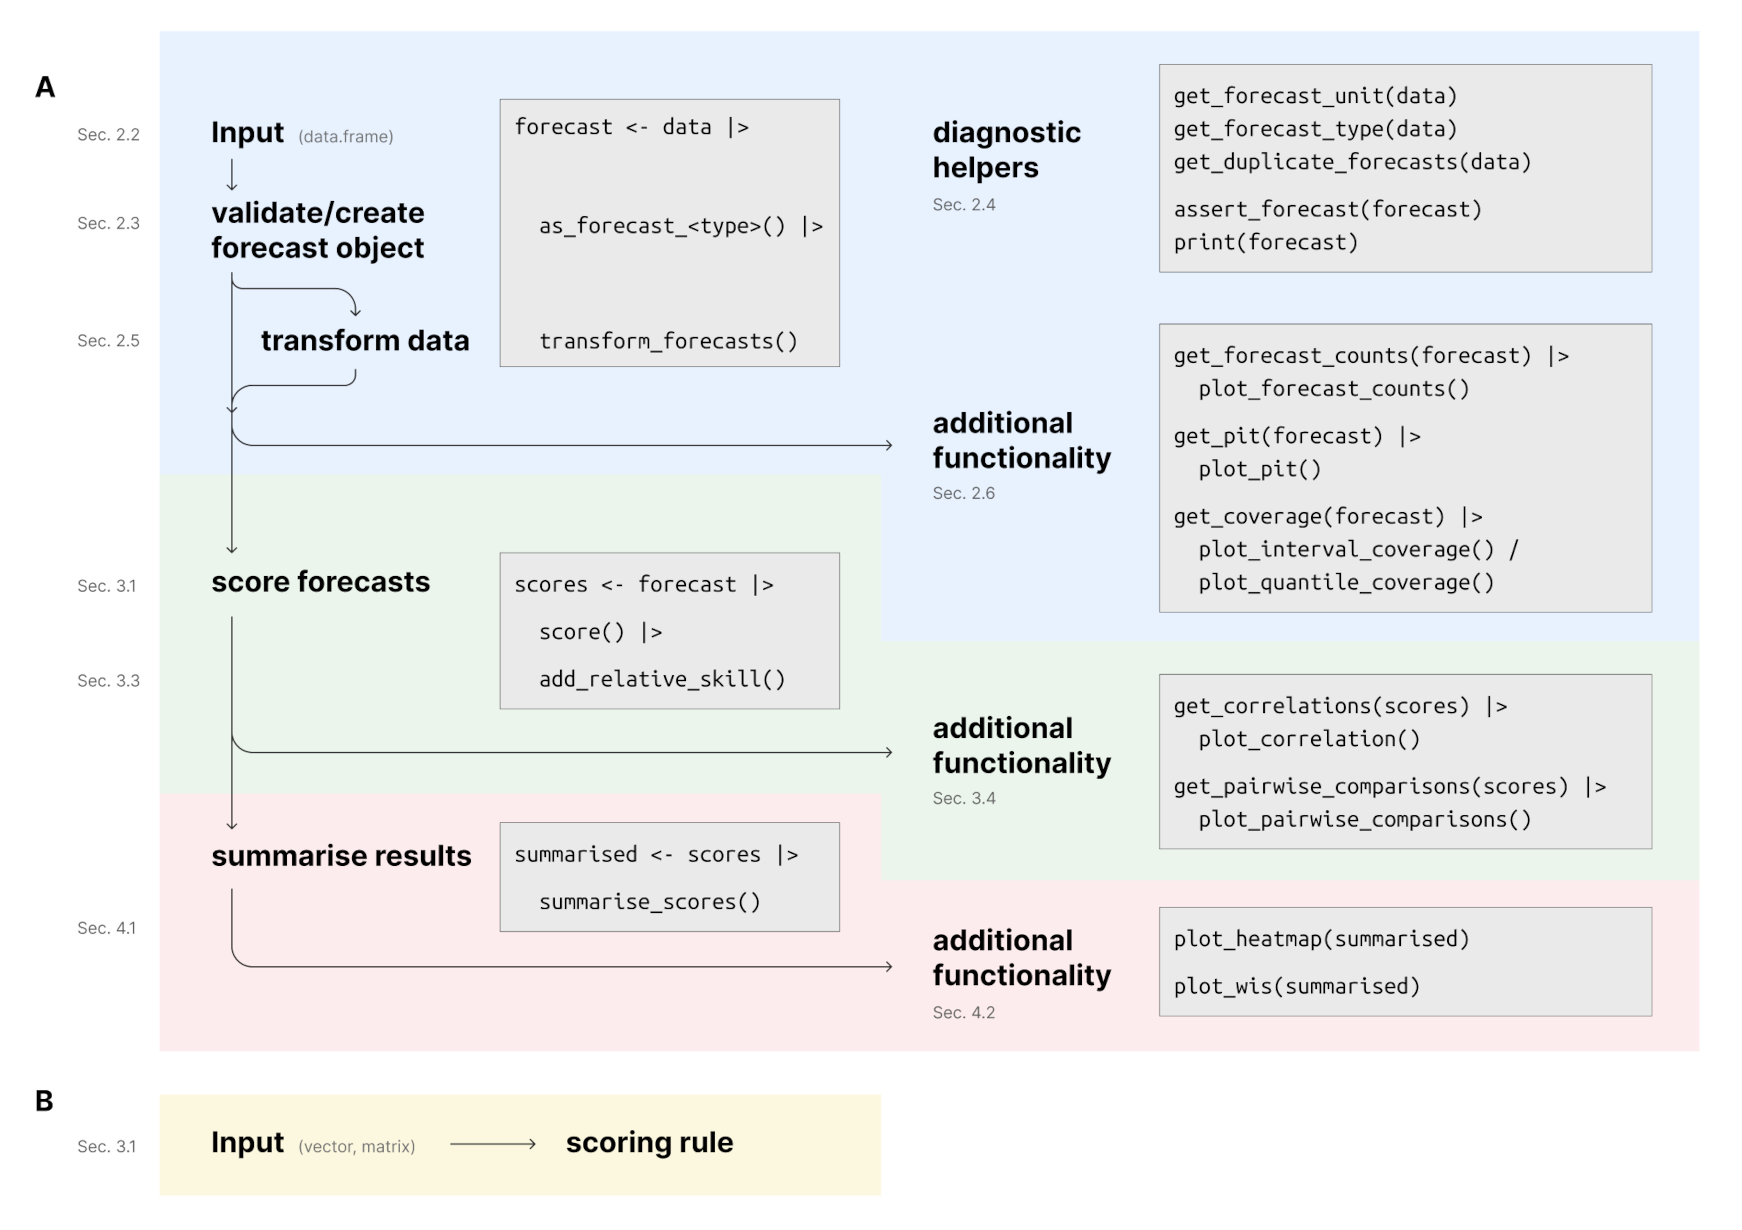
\includegraphics[width=1\linewidth]{output/workflow} 

}

\caption[Illustration of the workflow for working with scoringutils]{Illustration of the workflow for working with scoringutils.}\label{fig:workfklow-scoringutils}
\end{figure}
\end{CodeChunk}

\subsection{Forecast types}\label{forecast-types}

Forecasts differ in the exact prediction task and in how the forecaster
chooses to represent their prediction. To distinguish different kinds of
forecasts, \texttt{scoringutils} uses the term ``forecast type'' (which
is more a convenient classification than a formal definition). At the
moment, \texttt{scoringutils} distinguishes four different forecast
types: ``binary'', ``point'', ``quantile'' and ``sample'' forecasts
(support for more forecast types is planned for the future).

``Binary'' denotes a probability forecast for a binary (yes/no) outcome
variable. This is sometimes also called ``soft binary classification''.
``Point'' denotes a forecast for a continuous or discrete outcome
variable that is represented by a single number. ``Quantile'' or
``quantile-based'' is used to denote a probabilistic forecast for a
continuous or discrete outcome variable, with the forecast distribution
represented by a set of predictive quantiles. While a single quantile
would already satisfy the requirements for a quantile-based forecast,
most scoring rules expect a set of quantiles which are symmetric around
the median (thus forming the lower and upper bounds of central
``prediction intervals'') and will return \texttt{NA} if this is not the
case. ``Sample'' or ``sample-based'' is used to denote a probabilistic
forecast for a continuous or discrete outcome variable, with the
forecast represented by a finite set of samples drawn from the
predictive distribution. A single sample technically suffices, but would
to very imprecise results.

Forecast types (in the \texttt{data.frame} framework) are determined
based on the names and the type of the columns present in the input.
Table \ref{fig:input-score} shows the expected input format for each
forecast type. Forecast types that are planned, but not currently
supported, are greyed out. Input formats for the scoring rules that can
be called directly follow the same convention, with inputs expected to
be vectors or matrices.

\begin{CodeChunk}
\begin{figure}[!h]

{\centering \includegraphics[width=1\linewidth]{output/input-score} 

}

\caption[Table with different input formats]{Table with different input formats.}\label{fig:input-score}
\end{figure}
\end{CodeChunk}

\subsection{Classes}\label{classes}

\pkg{scoringutils} uses separate classes that correspond to the
different forecast types. Those are currently \texttt{forecast\_binary},
\texttt{forecast\_point}, \texttt{forecast\_quantile}, and
\texttt{forecast\_sample}. These classes are used to allow for dedicated
input checks and sensible defaults for the scoring rules to be applied
to the forecasts.

They come with a constructor, \code{new\_forecast()}, a generic
validator, \code{validate\_forecast()} (which dispatches to a
specialised validator method depending on the class of the input), and a
convenient wrapper function \code{as\_forecast()}. \code{as\_forecast()}
determines the forecast type of the input, constructs the class and
validates the input. The process is illustrated in Figure
\ref{fig:flowchart-validation}. All classes also have a \texttt{print()}
method designed to provide helpful information to the user.

\begin{CodeChunk}
\begin{figure}[!h]

{\centering \includegraphics[width=1\linewidth]{output/flowchart-create-object} 

}

\caption[Illustration of the process of creating a `forecast` object]{Illustration of the process of creating a `forecast` object.}\label{fig:flowchart-validation}
\end{figure}
\end{CodeChunk}

\subsection{Example data}\label{example-data}

The example data included in the package and used in this paper consists
of one to three week ahead forecasts made between May and September 2021
for COVID-19 cases and deaths from four different forecasting models. It
represents a small subset of short-term predictions for COVID-19 cases
and deaths submitted to the European Forecast Hub
\citep{europeancovid-19forecasthubEuropeanCovid19Forecast2021}. One to
four week ahead predictions of different COVID-19 related targets were
submitted to the Forecast Hub each week in a quantile-based format. The
full official hub evaluations, which also use \pkg{scoringutils}, can be
seen at \url{https://covid19forecasthub.eu/}. The example data was
converted to all the different forecast types used in
\pkg{scoringutils}, in order to illustrate the workflows and provide
users with a reference for the correct input formats. The example data
also contains observations without corresponding forecasts, both for the
purposes of plotting the data and to make the example data more
realistic. The stored data sets are called \texttt{example\_quantile},
\texttt{example\_continuous}, \texttt{example\_integer},
\texttt{example\_point} and \texttt{example\_binary}.

Here is the output of validating the example data:

\begin{CodeChunk}
\begin{CodeInput}
R> library(scoringutils)
R> print(example_quantile, 2)
\end{CodeInput}
\begin{CodeOutput}
       location target_end_date target_type observed location_name
    1:       DE      2021-01-02       Cases   127300       Germany
    2:       DE      2021-01-02      Deaths     4534       Germany
   ---                                                            
20544:       IT      2021-07-24      Deaths       78         Italy
20545:       IT      2021-07-24      Deaths       78         Italy
       forecast_date quantile predicted                model horizon
    1:          <NA>       NA        NA                 <NA>      NA
    2:          <NA>       NA        NA                 <NA>      NA
   ---                                                              
20544:    2021-07-12    0.975       611 epiforecasts-EpiNow2       2
20545:    2021-07-12    0.990       719 epiforecasts-EpiNow2       2
\end{CodeOutput}
\begin{CodeInput}
R> validated <- validate(example_quantile) 
R> class(validated)
\end{CodeInput}
\begin{CodeOutput}
[1] "scoringutils_quantile" "data.table"           
[3] "data.frame"           
\end{CodeOutput}
\end{CodeChunk}

\subsection{Diagnostic functions that provide additional information
about the
data}\label{diagnostic-functions-that-provide-additional-information-about-the-data}

In addition to printing the validated objects, users can call a variety
of different functions to obtain more information about the data and to
visualise it. Functions that provide this kind of additional information
usually are named starting with \texttt{get\_}.

\code{get\_forecast\_type()} infers the forecast type from a
\texttt{data.frame} and returns a single string (one of ``binary'',
``point'', ``sample'' or ``quantile''). \code{get\_forecast\_unit()}
returns a vector with the names of the columns that uniquely define a
single forecast (see Section \ref{sec:forecastunit} below for more
information).

\code{get\_forecast\_counts()} returns forecast counts, which is helpful
to obtain an overview of missing forecasts. This can impact the
evaluation, if missingness correlates with performance. Users can
specify the level of summary through the \texttt{by} argument. For
example, to see how many forecasts there are per model and target\_type,
we can run

\begin{CodeChunk}
\begin{CodeInput}
R> forecast_counts <- available_forecasts(
+   example_quantile, by = c("model", "target_type", "forecast_date")
+ )
\end{CodeInput}
\end{CodeChunk}

This returns an object of class \texttt{forecast\_counts}. We can
visualise the results by calling \code{plot()} on the object (Figure
\ref{fig:plot-forecast-counts}).

\begin{CodeChunk}
\begin{CodeInput}
R> library(ggplot2)
R> plot(forecast_counts, xvar = "forecast_date") + 
+   facet_wrap(~ target_type) + 
+   labs (y = "Model", x = "Forecast date")
\end{CodeInput}
\begin{figure}[!h]

{\centering 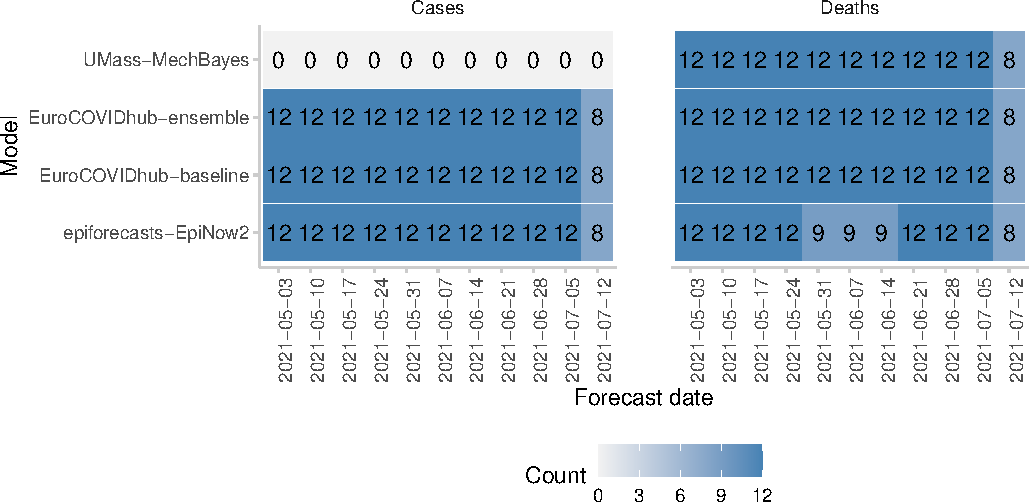
\includegraphics[width=1\linewidth]{manuscript_files/figure-latex/plot-forecast-counts-1} 

}

\caption[Forecast counts for the example data]{Forecast counts for the example data.}\label{fig:plot-forecast-counts}
\end{figure}
\end{CodeChunk}

\subsection{Visualising the data}\label{visualising-the-data}

Work in progress

\begin{CodeChunk}
\begin{CodeInput}
R> example_quantile %>%
+   make_na(what = "truth", 
+           target_end_date > "2021-07-15",
+           target_end_date <= "2021-05-22") %>%
+   make_na(what = "forecast", 
+           model != "EuroCOVIDhub-ensemble",
+           forecast_date != "2021-06-28") %>%
+   plot_predictions(x = "target_end_date", by = c("target_type", "location")) +
+   aes(colour = model, fill = model) +
+   facet_wrap(target_type ~ location, ncol = 4, scales = "free_y") +
+   labs(x = "Target end date")
\end{CodeInput}
\end{CodeChunk}

\section{Scoring forecasts}\label{scoring-forecasts}

\pkg{scoringutils} offers two ways of scoring forecasts: Users can
either call different scoring rules directly on vectors and matrices or
use the function \texttt{score()} on a data.frame (or similar) to apply
multiple scoring rules at once.

\subsection{score()}\label{score}

The \code{score()} is the workhorse of the package. It takes as input
either an object of class \texttt{forecast\_*} or a \texttt{data.frame}
(or similar) with forecasts, as well as a list of functions (the scoring
rules). The function then applies those scoring rules to the input.
Additional arguments can be passed down to the scoring rules via
\texttt{...}. \code{score()} is a generic function that dispatches to
different methods depending on the class of the input.

\code{score.default()} is the default method that is used if
\code{as\_forecast()} has not yet been called on the input.
\code{score.default()} calls \code{as\_forecast()} and then calls
\code{score()} again in order to dispatch to the appropriate method. The
method then validates the input again, applies the scoring rules, and
returns a \texttt{data.table} with the scores. The process is
illustrated in Figure \ref{fig:flowchart-score}.

\begin{CodeChunk}
\begin{figure}[!h]

{\centering \includegraphics[width=1\linewidth]{output/flowchart-score} 

}

\caption[Flowchart for calling `score()`]{Flowchart for calling `score()`}\label{fig:flowchart-score}
\end{figure}
\end{CodeChunk}

\subsection{Scoring rules}\label{scoring-rules}

Scoring rules are the functions the various scores and metrics. They are
consistently named \texttt{name\ of\ the\ metric} + \_ +
\texttt{forecast\ type}. The return value is a vector with scores (only
in the case of \code{wis()} is there an optional argument that causes
the function to return a list of vectors). The first argument of a
scoring rule is always \texttt{observed}, and the second one is
\texttt{predicted}. Scoring rules for quantile-based arguments require
an additional vector that denotes the quantile levels of the predictive
quantiles.

Scoring rules differ in the relationship between input and output. Some
scoring rules have a one-to-one relationship between prediction and
score, returning one value per value in \texttt{predicted}. This is the
case for all scoring rules for binary and point forecasts. Other scoring
rules have a many-to-one relationship, returning one value per multiple
values in \texttt{predicted}. This is the case for all scoring rules for
sample- and quantile-based forecasts. For sample- and quantile-based
forecasts, \texttt{predicted} is therefore a matrix, with values in each
row jointly forming a single forecast.

Input formats and return values are shown in more detail in Figure
\ref{fig:input-scoring-rules}.

\begin{CodeChunk}
\begin{figure}[!h]

{\centering 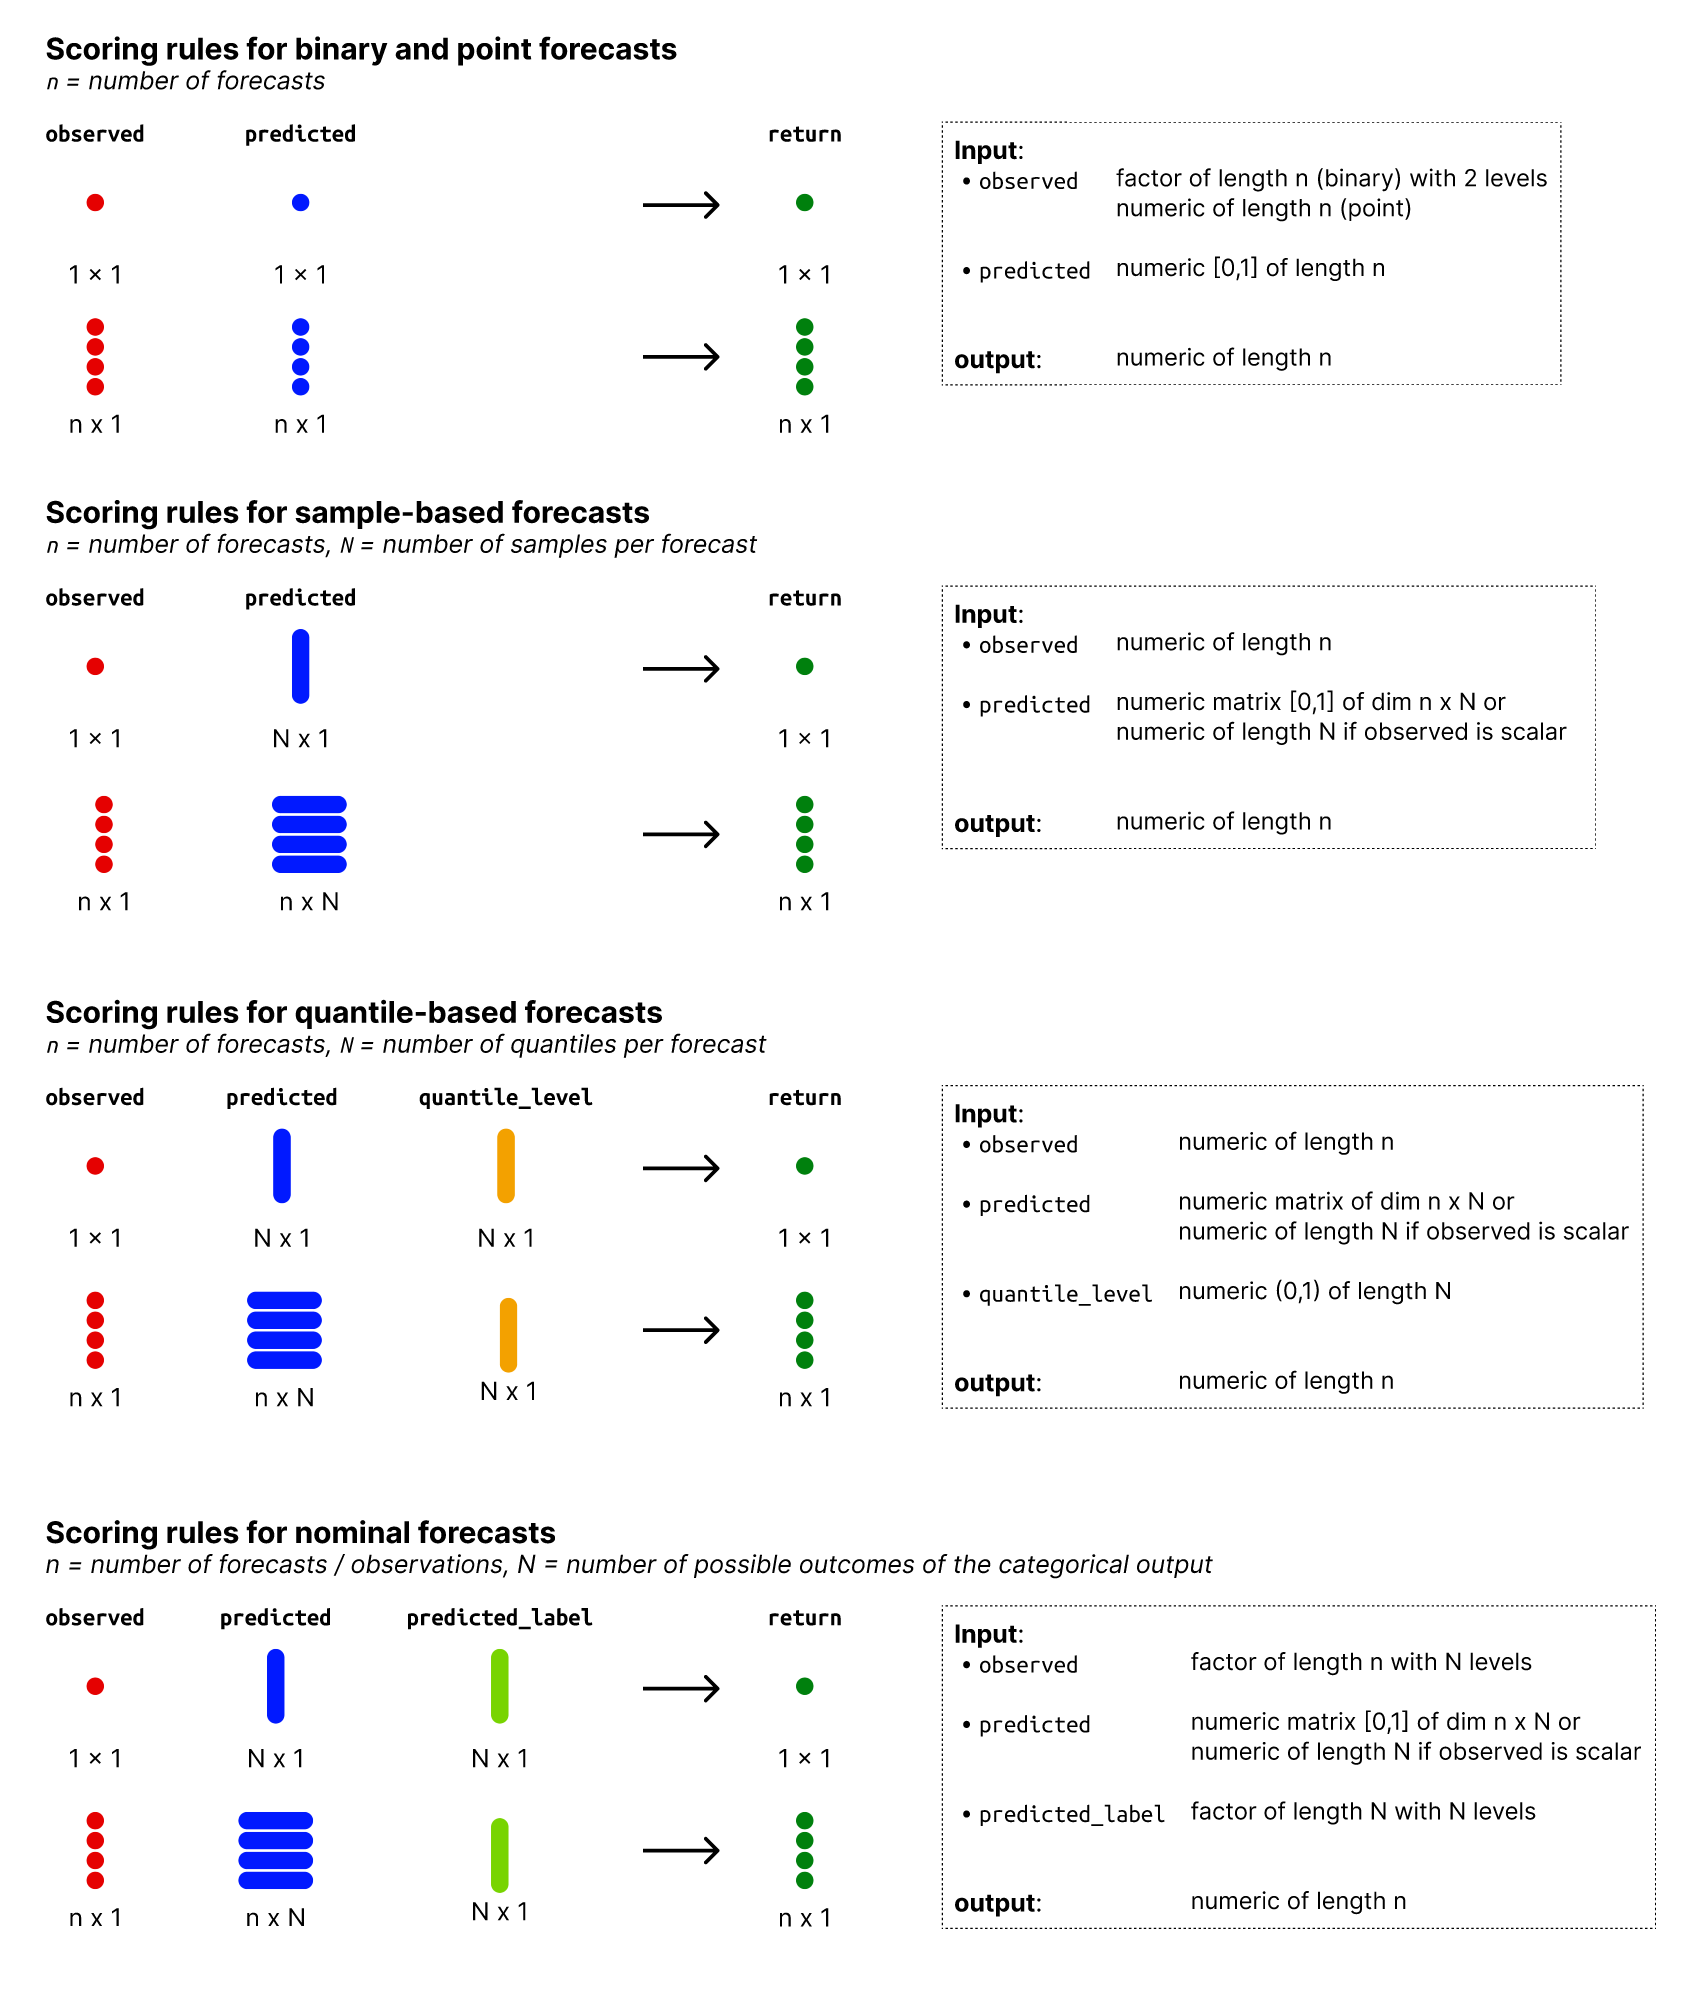
\includegraphics[width=1\linewidth]{output/input-formats-scoring-rules} 

}

\caption[Overview of the inputs and outputs of the scoring rules (scoring functions that can be called directly on a set of vectors / matrices)]{Overview of the inputs and outputs of the scoring rules (scoring functions that can be called directly on a set of vectors / matrices)}\label{fig:inputs-scoring-rules}
\end{figure}
\end{CodeChunk}

\subsection{Passing scoring rules to
score()}\label{passing-scoring-rules-to-score}

The second argument to \code{score()} is a named list of scoring rules.
Names of the list item will be used as names of the columns in the
output corresponding to the respective scoring rule. The default list
for every forecast type can be accessed by calling
\code{metrics_binary()}, \code{metrics_point()},
\code{metrics\_sample()} and \code{metrics\_quantile()}.

Scoring rules need to be compatible with the type of the forecast that
is scored and need to have compatible input formats and return values.
Within \code{score()}, arguments are passed by position, meaning that
users are not tied to the \pkg{scoringutils} naming convention, and can
supply functions that take equivalent, but differently called arguments.
The default metrics for point forecasts, for example, uses functions
from the \pkg{Metrics} package, which use the names \texttt{actual} and
\texttt{predicted} instead of \texttt{observed} and \texttt{predicted}.

\begin{CodeChunk}
\begin{CodeInput}
R> score(example_point) |>
+   print(2)
\end{CodeInput}
\begin{CodeOutput}
     location target_end_date target_type observed location_name
  1:       DE      2021-05-08       Cases   106987       Germany
  2:       DE      2021-05-08       Cases   106987       Germany
 ---                                                            
886:       IT      2021-07-24      Deaths       78         Italy
887:       IT      2021-07-24      Deaths       78         Italy
     forecast_date predicted                 model horizon ae_point
  1:    2021-05-03    119258 EuroCOVIDhub-ensemble       1    12271
  2:    2021-05-03    132607 EuroCOVIDhub-baseline       1    25620
 ---                                                               
886:    2021-07-05       104  epiforecasts-EpiNow2       3       26
887:    2021-07-12       186  epiforecasts-EpiNow2       2      108
      se_point       ape
  1: 150577441 0.1146962
  2: 656384400 0.2394683
 ---                    
886:       676 0.3333333
887:     11664 1.3846154
\end{CodeOutput}
\end{CodeChunk}

\subsection[The unit of a single forecast]{The unit of a single
forecast}\label{sec:forecastunit}

In order to score forecasts, \pkg{scoringutils} needs to know which of
the rows of the data belong together and jointly form a single
forecasts. This is easy e.g.~for point forecast, where there is one row
per forecast. Probabilistic forecasts, however, are usually composed of
several values and for quantile or sample-based forecasts, there are
therefore multiple rows that belong to a single forecast.

The unit of a single forecast (or ``forecast unit'') is defined by the
other columns of the data (except for a few protected columns). A single
forecast should be uniquely defined by the combination of values in
those columns. For example, consider forecasts made by different models
in various locations at different time points and for different targets.
A single forecast could then be uniquely described by the values in the
columns ``model'', ``location'', ``date'', and ``target'', and the
forecast unit would be
\texttt{forecast\_unit\ =\ c("model",\ "location",\ "date",\ "taret")}.
As the forecast unit is internally determined based on the names of the
existing columns, it is mandatory that no column is present that is
unrelated to the forecast unit. As a very simplistic example, consider
an additional row, ``even'', that is one if the row number is even and
zero otherwise. The existence of this column would change results, as
\code{score()} assumes it was relevant to grouping the forecasts.

In order to avoid issues, we recommend using the function
\code{set\_forecast\_unit()} to determine the forecast unit manually.
The function simply drops unneeded columns, while making sure that all
necessary, `protected columns' like \texttt{predicted} or
\texttt{observed} are retained. You can get a list of all protected
columns by calling \code{get\_protected\_columns()}. You can get the
current forecast unit by calling \code{get\_forecast\_unit()} on the
data or by simply printing the object if it is of class
\texttt{forecast\_*}.

The function \code{get\_duplicate\_forecasts()} may be helpful in case
\code{validate\_forecast()} returns an error message about duplicate
forecasts. This can occur if there is more than one predicted value for
a single forecast unit. In the case of quantile- and sample-based
forecasts, rows will only be considered duplicates if they have the same
quantile level or sample id. Duplicate forecasts can be a sign of a
wrongly defined forecast unit. For example, if we dropped the column
\texttt{target\_type} in the example data, we would obtain an error
about duplicate forecasts. Even though the predicted values differ,
there are now two different forecasts for the exact same forecast unit,
as far as \pkg{scoringutils} can tell.
\code{get\_duplicate\_forecasts()} finds duplicates and returns them for
the user to inspect.

\begin{CodeChunk}
\begin{CodeInput}
R> rbind(example_quantile, example_quantile[1001:1002]) |>
+   get_duplicate_forecasts() 
\end{CodeInput}
\begin{CodeOutput}
   location target_end_date target_type observed location_name
1:       DE      2021-05-22      Deaths     1285       Germany
2:       DE      2021-05-22      Deaths     1285       Germany
3:       DE      2021-05-22      Deaths     1285       Germany
4:       DE      2021-05-22      Deaths     1285       Germany
   forecast_date quantile predicted                model horizon
1:    2021-05-17    0.975      1642 epiforecasts-EpiNow2       1
2:    2021-05-17    0.990      1951 epiforecasts-EpiNow2       1
3:    2021-05-17    0.975      1642 epiforecasts-EpiNow2       1
4:    2021-05-17    0.990      1951 epiforecasts-EpiNow2       1
\end{CodeOutput}
\end{CodeChunk}

\subsection{Transforming forecasts}\label{transforming-forecasts}

As suggested in \citep{bosseScoringEpidemiologicalForecasts2023}, users
may want to transform forecasts before scoring them. In an
epidemiological context for example, the continuous ranked probability
score (CRPS) and the weighted interval score (WIS) are two commonly used
scoring rules. Both measure the absolute distance between the forecast
and the observation. This may not be desirable in the context of
epidemiological forecasts, where infectious disease processes are
usually modelled to occur on a multiplicative scale. Taking the
logarithm of the forecasts and observations before scoring them makes it
possible to evaluate forecasters based on how well they predicted the
exponential growth rate.

The function \code{transform\_forecasts()} allows users to apply
arbitrary transformations to forecasts and observations. Users can
specify a function via the argument \code{fun} (as well as supply
additional function parameters). The default function is
\code{log_shift()}, which is simply a wrapper around \code{log()} with
an additional offset to deal with zeroes in the data, i.e.~computing
\code{log(x + offset)}. Users can specify to either append the
transformed forecasts to the existing data by setting
\code{append = TRUE} (the default behaviour, resulting in an additional
column \texttt{scale}) or to replace the existing forecasts in place.

Before calling the logarithm, we need to make sure that there are no
negative values in the data. When evaluating forecasts of
epidemiological count data, one should perhaps simply remove negative
observations altogether, but for illustrative purposes we will replace
them with zeroes first before appending transformed counts.

\begin{CodeChunk}
\begin{CodeInput}
R> example_quantile |> 
+   transform_forecasts(fun = \(x) {pmax(x, 0)}, append = FALSE) |>
+   transform_forecasts(fun = log_shift, offset = 1) |>
+   print(2)
\end{CodeInput}
\begin{CodeOutput}
       location target_end_date target_type     observed
    1:       DE      2021-01-02       Cases 1.273000e+05
    2:       DE      2021-01-02      Deaths 4.534000e+03
   ---                                                  
41089:       IT      2021-07-24      Deaths 4.369448e+00
41090:       IT      2021-07-24      Deaths 4.369448e+00
       location_name forecast_date quantile predicted
    1:       Germany          <NA>       NA        NA
    2:       Germany          <NA>       NA        NA
   ---                                               
41089:         Italy    2021-07-12    0.975  6.416732
41090:         Italy    2021-07-12    0.990  6.579251
                      model horizon   scale
    1:                 <NA>      NA natural
    2:                 <NA>      NA natural
   ---                                     
41089: epiforecasts-EpiNow2       2     log
41090: epiforecasts-EpiNow2       2     log
\end{CodeOutput}
\end{CodeChunk}

\subsection{Summarising scores}\label{summarising-scores}

Usually, users will not be interested in the scores for each individual
forecast, but rather in a summarised score. The function
\code{summarise\_scores()} allows users to aggregate scores across
dimensions using an arbitrary function.

There are two different, but essentially equivalent ways of specifying
the summary level. Users can either specify the columns that should be
retained (using the argument \texttt{by}), or they can specify the
columns that should be aggregated over (using the argument
\code{across}).

\begin{CodeChunk}
\begin{CodeInput}
R> example_quantile[horizon == 2] |>
+   score(metrics = list("wis" = wis)) |>
+   summarise_scores(by = c("model", "target_type"))
\end{CodeInput}
\end{CodeChunk}

Summarised scores can then be visualised using the function
\code{XXXscores\_table()}. In order to display scores it is often useful
to round the output, for example to two significant digits, which can be
achieved with another call to \code{summarise\_scores()}. The output of
the following is shown in Figure \ref{fig:score-table}:

\begin{CodeChunk}
\begin{CodeInput}
R> example_quantile[horizon == 2] |>
+   score() |>
+   summarise_scores(by = c("model", "target_type")) |>
+   summarise_scores(fun = signif, digits = 2) |>
+   plot_score_table(y = "model", by = "target_type") + 
+   facet_wrap(~ target_type)
\end{CodeInput}
\begin{figure}

{\centering 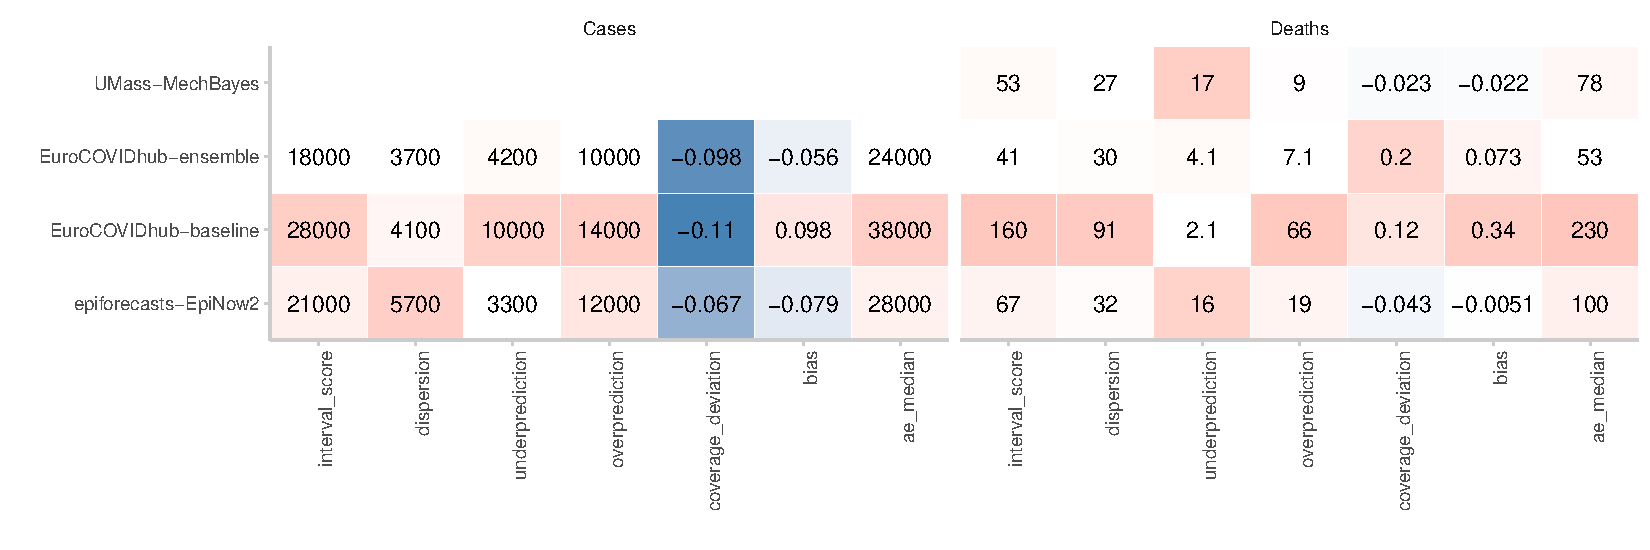
\includegraphics[width=1\linewidth]{manuscript_files/figure-latex/score-table-1} 

}

\caption[Coloured table to visualise the computed scores]{Coloured table to visualise the computed scores. Red colours indicate that a value is higher than ideal, blue indicates it is lower than ideal and the opacity indicates the strength of the deviation from the ideal.}\label{fig:score-table}
\end{figure}
\end{CodeChunk}

While \code{summarise\_scores()} accepts arbitrary summary functions,
care has to be taken when using something else than \code{mean()}. Many
scoring rules for probabilistic forecasts are so-called `strictly proper
scoring rules' \citep{gneitingStrictlyProperScoring2007}. Strictly
proper scoring rules are constructed such that they cannot always
incentivise the forecaster to report her honest belief about the future
and cannot be cheated. Let's assume that a forecaster's true belief
about the future corresponds to a predictive distribution \(F\). Then,
if \(F\) really was the true data-generating process, a scoring rule
would be proper if it ensures that no other forecast distribution \(G\)
would yield a better expected score. If the scoring rule ensures that
under \(F\) no other possible predictive distribution can achieve the
same expected score as \(F\), then it is called strictly proper. From
the forecaster's perspective, any devation from her true belief \(F\)
leads to a worsening of expected scores. When using summary functions
other then the mean, however, scores may lose their propriety (the
property of incentivising honest reporting) and become cheatable. For
example, the median of several individual scores (individually based on
a strictly roper scoring rule) is usually not proper. A forecaster
judged by the median of several scores may be incentivised to
misrepresent their true belief in a way that is not true for the mean
score.

The user must exercise additional caution and should usually avoid
aggregating scores across categories which differ much in the magnitude
of the quantity to forecast, as forecast errors usually increase with
the order of magnitude of the forecast target. In the given example,
looking at one score per model (i.e., specifying
\code{summarise_by = c("model")}) is problematic, as overall aggregate
scores would be dominated by case forecasts, while performance on deaths
would have little influence. Similarly, aggregating over different
forecast horizons is often ill-advised as the mean will be dominated by
further ahead forecast horizons. In the previous function calls, we
therefore decided to only analyse forecasts with a forecast horizon of
two weeks.

\subsection{Additional visualisations of
scores}\label{additional-visualisations-of-scores}

\subsubsection{Heatmaps}\label{heatmaps}

To detect systematic patterns it may be useful to visualise a single
metric across several dimensions. The function \code{plot\_heatmap()}
can be used to create a heatmap that achieves this. The following
produces a heatmap of bias values across different locations and
forecast targets (output shown in Figure \ref{fig:score-heatmap}).

\begin{CodeChunk}
\begin{CodeInput}
R> score(example_continuous) |>
+   summarise_scores(by = c("model", "location", "target_type")) |>
+   plot_heatmap(x = "location", metric = "bias") + 
+     facet_wrap(~ target_type) 
\end{CodeInput}
\begin{figure}[!h]

{\centering 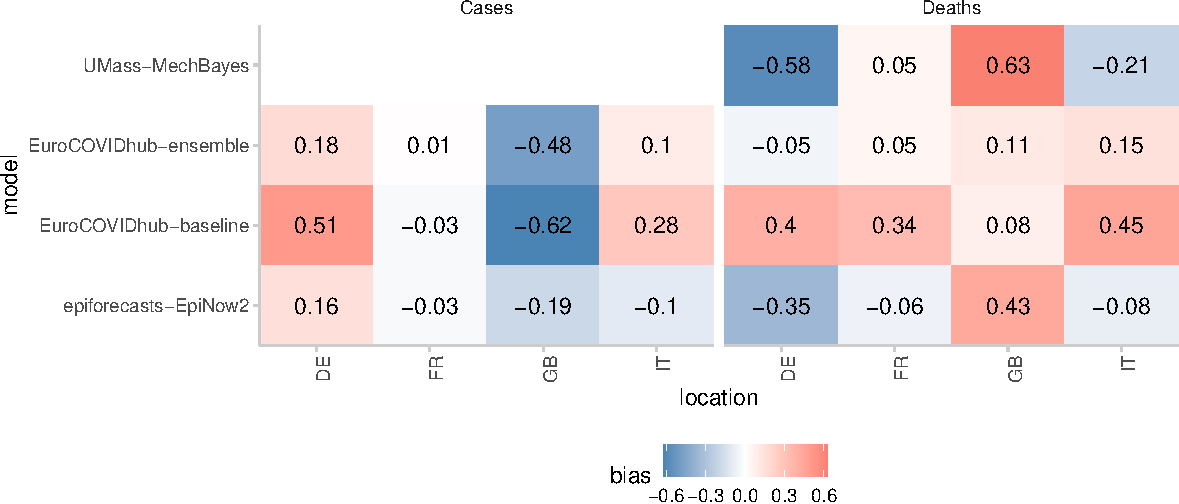
\includegraphics[width=1\linewidth]{manuscript_files/figure-latex/score-heatmap-1} 

}

\caption[Heatmap of bias values for different models across different locations and forecast targets]{Heatmap of bias values for different models across different locations and forecast targets. Bias values are bound between -1 (underprediction) and 1 (overprediction) and should be 0 ideally. Red tiles indicate an upwards bias (overprediction), while blue tiles indicate a downwards bias (under-predicction)}\label{fig:score-heatmap}
\end{figure}
\end{CodeChunk}

\subsubsection{Weighted interval score
decomposition}\label{weighted-interval-score-decomposition}

For quantile-based forecasts, the weighted interval score
\citep[WIS, ][]{bracherEvaluatingEpidemicForecasts2021} is commonly used
and is a strictly proper scoring rule. The WIS treats the predictive
quantiles as a set of symmetric prediction intervals and measures the
distance between the observation and the forecast interval. It can be
decomposed into a dispersion (uncertainty) component and penalties for
over- and underprediction. For a single interval, the interval score is
computed as
\[IS_\alpha(F,y) = \underbrace{(u-l)}_\text{dispersion} + \underbrace{\frac{2}{\alpha} \cdot (l-y) \cdot \mathbf{1}(y \leq l)}_{\text{overprediction}} + \underbrace{\frac{2}{\alpha} \cdot (y-u) \cdot \mathbf{1}(y \geq u)}_{\text{underprediction}}, \]
where \(\mathbf{1}()\) is the indicator function, \(y\) is the observed
value, and \(l\) and \(u\) are the \(\frac{\alpha}{2}\) and
\(1 - \frac{\alpha}{2}\) quantiles of the predictive distribution \(F\),
i.e.~the lower and upper bound of a single prediction interval. For a
set of \(K\) prediction intervals and the median \(m\), the score is
computed as a weighted sum,
\[WIS = \frac{1}{K + 0.5} \cdot \left(w_0 \cdot |y - m| + \sum_{k = 1}^{K} w_k \cdot IS_{\alpha}(F, y)\right),\]
where \(w_k\) is a weight for every interval. Usually,
\(w_k = \frac{\alpha_k}{2}\) and \(w_0 = 0.5\). It is helpful to
visualise the decomposition of the weighted interval score into its
components: dispersion, overprediction and underprediction. This can be
achieved using the function \code{plot\_wis()}, as shown in Figure
\ref{fig:wis-components}

\begin{CodeChunk}
\begin{CodeInput}
R> score(example_quantile) |>
+   summarise_scores(by = c("model", "target_type")) |>
+   plot_wis(relative_contributions = FALSE) + 
+   facet_wrap(~ target_type, 
+              scales = "free_x") 
\end{CodeInput}
\end{CodeChunk}

\begin{CodeChunk}
\begin{figure}[!h]

{\centering 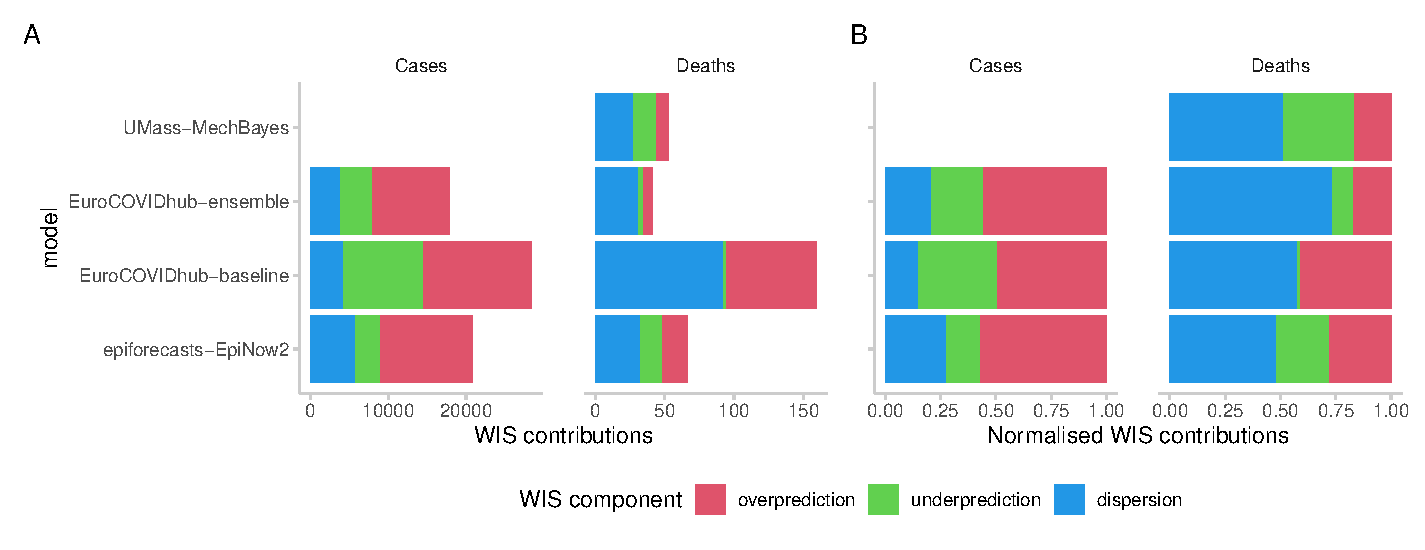
\includegraphics[width=1\linewidth]{manuscript_files/figure-latex/wis-components-1} 

}

\caption[Decomposition of the weighted interval score (WIS) into dispersion, overprediction and underprediction]{Decomposition of the weighted interval score (WIS) into dispersion, overprediction and underprediction. A: absolute contributions, B: contributions normalised to 1.}\label{fig:wis-components}
\end{figure}
\end{CodeChunk}

\subsection{Correlations}\label{correlations}

Users can examine correlations between scores using the function
\code{correlation()}. This produces an output of class XXX with its own
plot method. The plot resulting from the following code is shown in
Figure \ref{fig:correlation-plot}.

\begin{CodeChunk}
\begin{CodeInput}
R> correlations <- example_quantile |>
+   score() |>
+   summarise_scores() |>
+   correlation()
R> 
R> correlations |>
+   plot()
\end{CodeInput}
\begin{figure}[!h]

{\centering 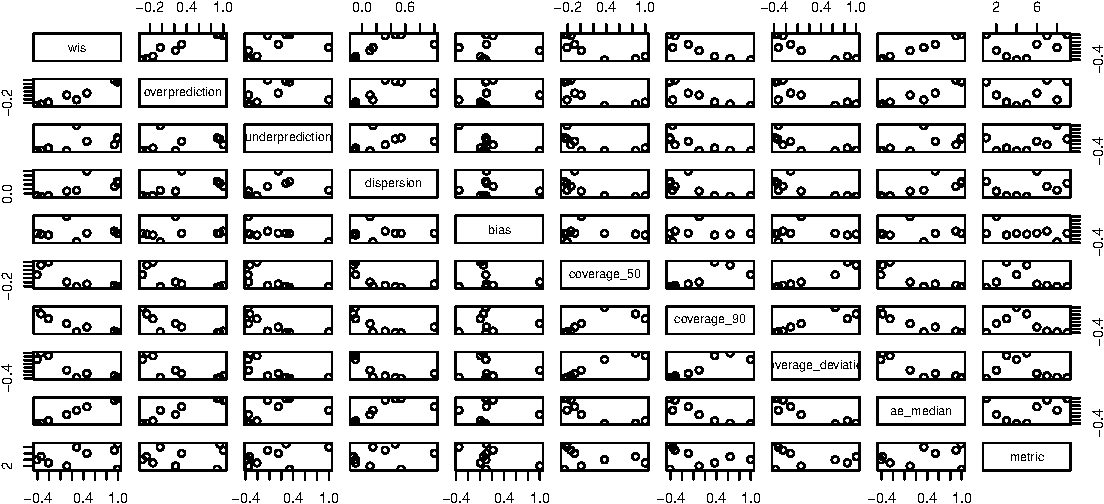
\includegraphics[width=1\linewidth]{manuscript_files/figure-latex/correlation-plot-1} 

}

\caption[Correlation between different scores]{Correlation between different scores}\label{fig:correlation-plot}
\end{figure}
\end{CodeChunk}

\subsection{Pairwise comparisons}\label{pairwise-comparisons}

\subsection{Pairwise comparisons}\label{pairwisetheory}

Raw scores for different forecasting models are not directly comparable
in the case of missing forecasts, as forecasting targets usually differ
in their characteristics (e.g., the scale of the forecast target, how
difficult targets are to forecast etc.). One way to mitigate this are
relative skill scores based on pairwise comparisons
\citep{cramerEvaluationIndividualEnsemble2021}.

Models enter a `pairwise tournament', where all possible pairs of models
are compared based on the overlapping set of available forecasts common
to both models (omitting comparisons where there is no overlapping set
of forecasts). For every pair, the ratio of the mean scores of both
models is computed. The relative skill score of a model is then the
geometric mean of all mean score ratios which involve that model. This
gives us an indicator of performance relative to all other models, with
the orientation depending on the score used (if lower values are better
for a particular scoring rule, then the same is true for the relative
skill score computed based on that score). Two models can of course only
be fairly compared if they have overlapping forecasts. One simple rule
of thumb one could apply is to only compare models that have forecasts
for at least 50\% of the available targets, thereby ensuring that all
models have overlapping sets of forecasts. Furthermore, pairwise
comparisons between models for a given metric are only possible if all
values have the same sign, i.e.~all score values need to be either
positive or negative. The process of pairwise comparisons is illustrated
in Figure \ref{fig:pairwise-comparison}.

\begin{CodeChunk}
\begin{figure}[!h]

{\centering \includegraphics[width=1\linewidth]{output/pairwise-comparisons} 

}

\caption[Illustration of the computation of relative skill scores through pairwise comparisons of three different forecast models, M1-M3.]{Illustration of the computation of relative skill scores through pairwise comparisons of three different forecast models, M1-M3..}\label{fig:pairwise-comparison}
\end{figure}
\end{CodeChunk}

Relative skill scores via pairwise comparisons can be calculated in two
different ways. The first one is by calling the function
\code{pairiwse\_comparison()}. It takes a \code{data.table} (or similar)
of scores as input, and returns a \code{data.table} with the results of
the pairwise tournament. It displays the mean scores ratio for every
pair of models, a p-value for whether scores for one model are
significantly different from scores for another model, and the relative
skill score for every model. Users can also specify a baseline model, in
which case a scaled relative skill scores is computed by dividing the
relative skill score of every model by the relative skill score of the
baseline model. Another option is to call the function
\code{add\_pairwise\_comparison()} on the output of \code{score()} which
will simply add additional columns for the relative skill and scaled
relative skill.

In both cases, pairwise comparisons are computed according to the
grouping specified in the argument \code{by}: internally, the
\code{data.table} with all scores gets split into different
\code{data.table}s according to the values specified in \code{by}
(excluding the column `model'). Relative scores are then computed for
every individual group separately. In the example below we specify
\code{by = c("model", "target_type")}, which means that there is one
relative skill score per model, calculated separately for the different
forecasting targets.

\begin{CodeChunk}
\begin{CodeInput}
R> s <- score(example_quantile[horizon == 2])
R> pairwise_comparison(s, by = c("model", "target_type")) |>
+   print(1:3)
\end{CodeInput}
\end{CodeChunk}

The output of \code{pairwise\_comparison()} is an object of class XXX
with its own \code{plot()} method. An example is shown in Figure
\ref{fig:pairwise-plot}.

\begin{CodeChunk}
\begin{CodeInput}
R> score(example_quantile) |>
+   pairwise_comparison(by = c("model", "target_type"), 
+                       baseline = "EuroCOVIDhub-baseline") |>
+   plot_pairwise_comparison() + 
+   facet_wrap(~ target_type)
\end{CodeInput}
\begin{figure}

{\centering 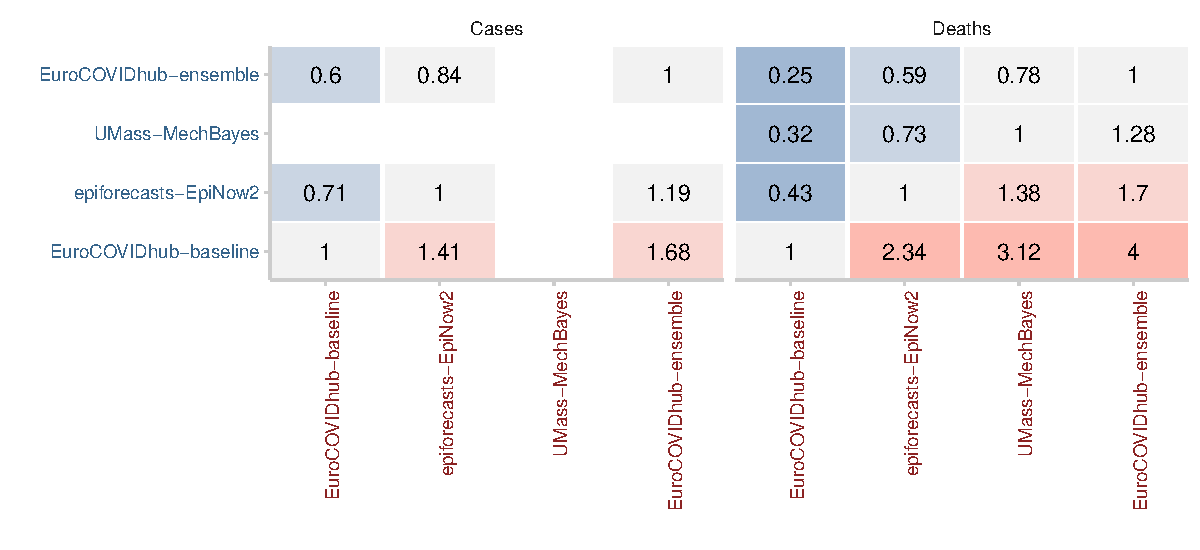
\includegraphics[width=1\linewidth]{manuscript_files/figure-latex/pairwise-plot-1} 

}

\caption[Ratios of mean weighted interval scores based on overlapping forecast sets]{Ratios of mean weighted interval scores based on overlapping forecast sets. When interpreting the plot one should look at the model on the y-axis, and the model on the x-axis is the one it is compared against. If a tile is blue, then the model on the y-axis performed better. If it is red, the model on the x-axis performed better in direct comparison. In the example above, the EuroCOVIDhub-ensemble performs best (it only has values smaller than one), while the EuroCOVIDhub-baseline performs worst (and only has values larger than one). For cases, the UMass-MechBayes model is excluded as there are no case forecasts available and therefore the set of overlapping forecasts is empty.}\label{fig:pairwise-plot}
\end{figure}
\end{CodeChunk}

It is in principle possible to compute p-values to determine whether two
models perform significantly differently. \pkg{scoringutils} allows to
compute these using either the Wilcoxon rank sum test (also known as
Mann-Whitney-U test) \citep{mannTestWhetherOne1947} or a permutation
test. In practice, this is complicated by the fact that both tests
assume independent observations. In reality, however, forecasts by a
model may be correlated across time or another dimension (e.g., if a
forecaster has a bad day, they might perform badly across different
targets for a given forecast date). P-values may therefore be too
liberal in suggesting significant differences where there aren't any.
One way to mitigate this is to aggregate observations over a category
where one suspects correlation (for example averaging across all
forecasts made on a given date) before making pairwise comparisons. A
test that is performed on aggregate scores will likely be more
conservative.

Pairwise comparisons should usually be made based on unsummarised scores
(the function \code{pairwise\_comparison()} internally summarises over
samples and quantiles automatically, but nothing else), as summarising
can change the set of overlapping forecasts between two models and
distort relative skill scores. When using \code{pairwise\_comparison()},
the function \code{summarise\_scores()} should therefore usually not be
called beforehand. One potential exception to this is when one is
interested in the p-values obtained from pairwise comparisons. As
forecasts are usually highly correlated (which the calculation of
p-values do not account for), it may be sensible to summaries over a few
categories (provided there are no missing values within the categories
summarised over) to reduce correlation and obtain more conservative
p-values.

\section{Calibration}\label{calibration}

Calibration refers to a statistical consistency (i.e., absence of
systematic deviations) between the forecasts and the observations. It is
possible to distinguish several forms of calibration which are discussed
in detail by \cite{gneitingProbabilisticForecastsCalibration2007}. The
form of calibration most commonly focused on is called probabilistic
calibration (for other form of calibration, see
\cite{gneitingProbabilisticForecastsCalibration2007}). Probabilistic
calibration means that the forecast distributions are consistent with
the true data-generating distributions in the sense that on average,
\(\tau\)\% of true observations will be below the corresponding
\(\tau\)-\%-quantiles of the cumulative forecast distributions.

\subsection{Interval coverage and quantile
coverage}\label{interval-coverage-and-quantile-coverage}

This of course, can be most easily verified for predictive distributions
in a quantile-based format. For such forecasts, one can easily compare
the proportion of observations that fall below the \(\tau\)-quantiles of
all forecasts (``empirical quantile coverage'') to the nominal quantile
coverage \(\tau\).

The above definition of probabilistic calibration also implies that the
empirical coverage of the central prediction intervals formed by the
predictive quantiles should be equal to the nominal interval coverage.
For example, the central 50\% prediction intervals of all forecasts
should really contain around 50\% of the observed values, the 90\%
central intervals should contain around 90\% of observations etc.
Forecasts that are too narrow and do not cover the required proportion
of observations are called overconfident or underdispersed, while
predictive distributions that are too wide are often called
underconfident, overdispersed or conservative.

Users can obtain coverage values for quantile-based predictions in two
different ways. The first is to call the functions XXX and XXX directly
as scoring rules within \texttt{score()} to obtain coverage values for
specific quantile-levels or central prediction intervals. A more
comprehensive way is by using the function \code{add\_coverage()}
directly on the raw forecasts. It adds additional columns with the width
of the central prediction interval corresponding to a given quantile
level, quantile coverage, interval coverage, quantile coverage deviation
and interval coverage deviation. Deviation here means the difference
between nominal and empirical coverage. Coverage for a single quantile
or interval is only ever \texttt{TRUE} or \texttt{FALSE}. Coverage
values are therefore only meaningful when summarised over many
forecasts. This can be done calling \texttt{summarise\_scores()}.
Results can then be visualised using the function
\texttt{plot\_interval\_coverage()} (see row 3 in Figure
\ref{fig:calibration-plots}) and \texttt{plot\_quantile\_coverage()}
(row 4 in Figure \ref{fig:calibration-plots}). Both show nominal against
empirical coverage. Ideally forecasters should lie on the diagonal line.
For interval coverage plots, a shift to the left means a forecaster is
too conservative and issues a predictive distribution that is too wide
and covers more of the observed values than needed. A shift to the right
means a forecaster is overconfident and the forecast distribution is too
narrow. For \emph{quantile coverage plots}, the interpretation depends
on whether the quantile is above or below the median. For quantiles
below the median, a line to the right of the diagonal (predictive
quantiles lower than the quantiles of the data-generating distribution)
means a forecaster is too conservative, while for quantiles above the
median, a line to the left of the diagonal line (predictive quantiles
higher than the quantiles of the data-generating distribution) implies
conservative predictions. Areas that imply a conservative forecaster are
shaded in green.

It is in principle possible to convert sample-based forecasts to
quantile-based forecasts using the function
\code{sample\_to\_quantile\_forecastXXX()} to make use of
\texttt{add\_coverage()}. This should be done with caution, as the
estimation of quantiles from predictive samples may be biased if the
number of available samples is not sufficiently large.

\subsection{Probability integral transform
(PIT)}\label{probability-integral-transform-pit}

A more natural way to visualise probabilistic calibration for
sample-based forecasts (and an alternative option for quantile-based
ones) is the probability integral transform (PIT) histogram
\citep{dawidPresentPositionPotential1984}.

Observed values, \(y\), are transformed using the CDF of the predictive
distribution, \(F\), to create a new variable \(u\) with \(u = F(y)\).
\(u\) is therefore simply the CDF of the predictive distribution
evaluated at the observed value. If forecasts are probabilistically
calibrated, then the transformed values will be uniformly distributed
(for a proof see for example
\citet{angusProbabilityIntegralTransform1994}). When plotting a
histogram of PIT values (see row 2 in Figure
\ref{fig:calibration-plots}), bias usually leads to a triangular shape,
a U-shaped histogram corresponds to forecasts that are under-dispersed
(too sharp) and a hump-shape appears when forecasts are over-dispersed
(too wide). There exist different variations of the PIT to deal with
discrete instead of continuous data (see
e.g.~\cite{czadoPredictiveModelAssessment2009} and
\cite{funkAssessingPerformanceRealtime2019}). The PIT version
implemented in \texttt{scoringutils} for discrete variables follows
\cite{funkAssessingPerformanceRealtime2019}.

\ldots and create PIT histograms using the function \code{plot\_pit()}.
The output of the following is shown in Figure \ref{fig:pit-plots}:

\begin{CodeChunk}
\begin{CodeInput}
R> example_continuous |>
+   pit(by = c("model", "target_type")) |>
+   plot_pit() + 
+   facet_grid(target_type ~ model)
\end{CodeInput}
\begin{figure}[!h]

{\centering 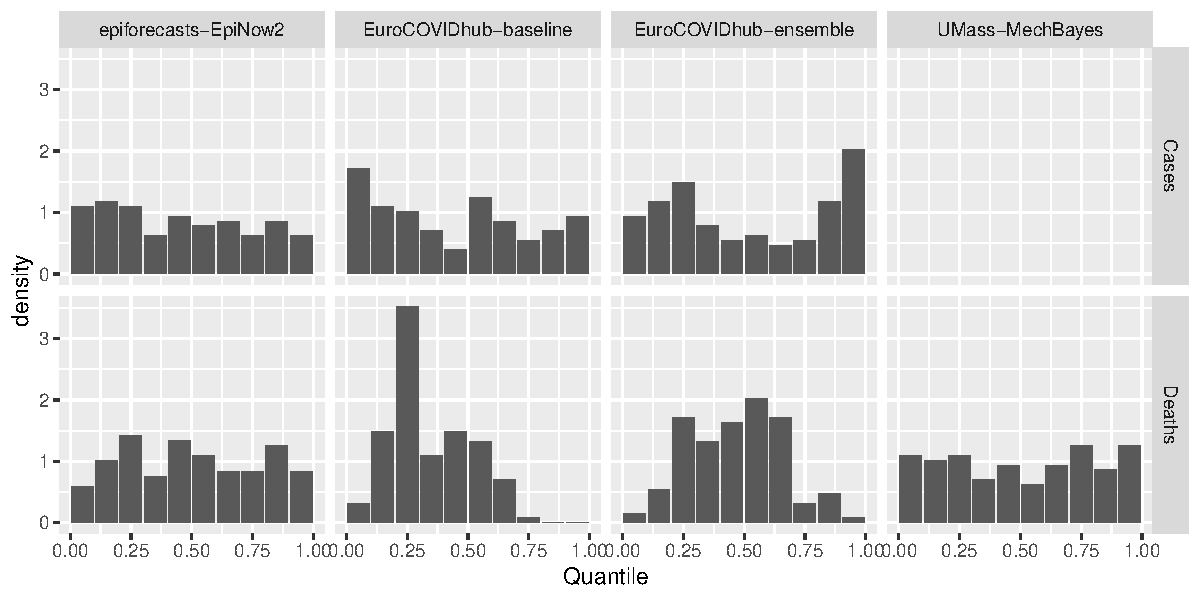
\includegraphics[width=1\linewidth]{manuscript_files/figure-latex/pit-plots-1} 

}

\caption[PIT histograms of all models stratified by forecast target]{PIT histograms of all models stratified by forecast target. Histograms should ideally be uniform. A u-shape usually indicates overconfidence (forecasts are too narrow), a hump-shaped form indicates underconfidence (forecasts are too uncertain) and a triangle-shape indicates bias.}\label{fig:pit-plots}
\end{figure}
\end{CodeChunk}

It is in theory possible to formally test probabilistic calibration, for
example by employing an Anderson Darling test on the uniformity of PIT
values. In practice this can be difficult as forecasts and therefore
also PIT values are often correlated. Personal experience suggests that
the Anderson Darling test is often too quick to reject the null
hypothesis of uniformity. It is also important to note that uniformity
of the PIT histogram (or a diagonal on quantile and interval coverage
plots) indicates probabilistic calibration, but does not guarantee that
forecasts are indeed calibrated in every relevant sense.
\cite{gneitingProbabilisticForecastsCalibration2007, hamillInterpretationRankHistograms2001a}
provide examples with different forecasters who are clearly
mis-calibrated, but have uniform PIT histograms.

\begin{CodeChunk}
\begin{figure}[!h]

{\centering \includegraphics[width=1\linewidth,]{output/calibration-diagnostic-examples} 

}

\caption[A]{A: Different forecasting distributions (black) against observations sampled from a standard normal distribution (grey histograms). B: PIT histograms based on the predictive distributions and the sampled observations shown in A. C: Empirical vs. nominal coverage of the central prediction intervals for simulated observations and predictions. Areas shaded in green indicate that the forecasts are too wide (i.e., underconfident), covering more true values than they actually should, while areas in white indicate that the model generates too narrow predictions and fails to cover the desired proportion of true values with its prediction intervals. D: Quantile coverage values, with green areas indicating too wide (i.e., conservative) forecasts. E: Scores for the standard normal predictive distribution and the observations drawn from different data-generating distributions.}\label{fig:calibration-plots}
\end{figure}
\end{CodeChunk}

\begin{CodeChunk}
\begin{CodeInput}
R> cov_scores <- score(example_quantile) |>
+   summarise_scores(by = c("model", "target_type", "range", "quantile"))
R> 
R> plot_interval_coverage(cov_scores) + 
+   facet_wrap(~ target_type)
R> 
R> plot_quantile_coverage(cov_scores) + 
+   facet_wrap(~ target_type)
\end{CodeInput}
\end{CodeChunk}

\begin{CodeChunk}
\begin{figure}[!h]

{\centering 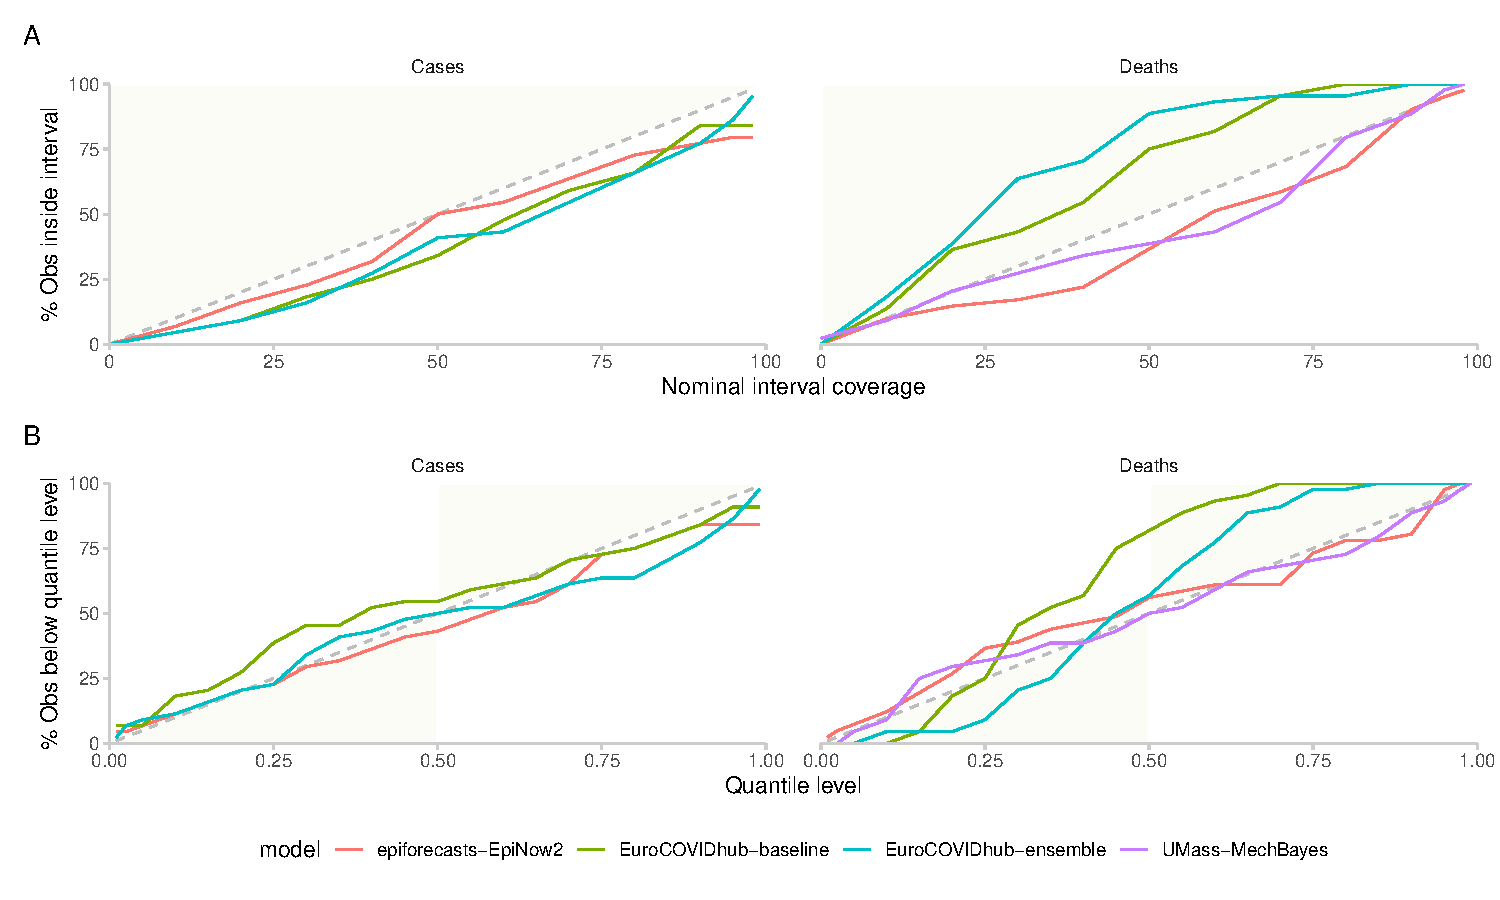
\includegraphics[width=1\linewidth]{manuscript_files/figure-latex/coverage-1} 

}

\caption[Interval coverage (A) and quantile coverage (B) plots]{Interval coverage (A) and quantile coverage (B) plots. Areas shaded in green indicate that the forecasts are too wide (i.e., underconfident), while areas in white indicate that the model is overconfident and generates too narrow predictions intervals.}\label{fig:coverage}
\end{figure}
\end{CodeChunk}

\subsection{Bias}\label{bias}

Another specific and very common form of miscalibration is bias,
i.e.~systematically over- or underpredicting the observed values.
\pkg{scoringutils} exports a bias metric \code{bias_quantile()} and
\code{bias_sample()}. The implementation follows
\cite{funkAssessingPerformanceRealtime2019} and captures how much
probability mass of the forecast was above or below the true value
(mapped to values between -1 and 1, with 0 being ideal). Values
represent a general tendency to over- or under-predict in relative
terms. A value of -1 implies that the entire probability mass of the
predictive distribution was below the observed value (and analogously
above it for a value of 1).

For forecasts in a quantile format, bias is also reflected in the over-
and underprediction components of the weighted interval score (a proper
scoring rule explained in more detail in Section \ref{wis}). These
measure over- and underprediction on an absolute scale (analogous to the
absolute error of a point forecast), rather than a relative scale. It is
important to note that it is not a priori clear what the decomposition
`should' look like - a forecast can be well calibrated and still have
different amounts of over- and underprediction. High overprediction or
underprediction values can therefore not immediately be interpreted as
systematic bias.

\section{Summary and discussion}\label{summary-and-discussion}

Future development plans

Forecast evaluation is invaluable to understanding and improving current
forecasts. The \pkg{scoringutils} package aims to facilitate this
process and make it easier, even for less experienced users. It provides
a fast, flexible and convenient evaluation framework based on
\texttt{data.frame}s, but also makes a set of scoring functions
available to more experienced users to be used in other packages or
pipelines. A set of visualisations and plotting functions help with
diagnosing issues with models and allow for thorough comparison between
different forecasting approaches.

The package is still under active development and we warmly welcome
contributions to \pkg{scoringutils}. In the future we hope to extend the
number of scoring metrics supported. This includes spherical scoring
rules
\citep{gneitingStrictlyProperScoring2007, joseCharacterizationSphericalScoring2009, macheteContrastingProbabilisticScoring2012},
evaluation of multinomial prediction tasks, as well as a broader range
of scoring metrics for point forecasts. We also plan to expand the
plotting functionality and hope to make templates available for
automated scoring reports.

\section{Acknowledgments}\label{acknowledgments}

Funding statements

NIB received funding from the Health Protection Research Unit (grant
code NIHR200908). HG MISSING. AC acknowledges funding by the NIHR, the
Sergei Brin foundation, USAID, and the Academy of Medical Sciences. EvL
acknowledges funding by the National Institute for Health Research
(NIHR) Health Protection Research Unit (HPRU) in Modelling and Health
Economics (grant number NIHR200908) and the European Union's Horizon
2020 research and innovation programme - project EpiPose (101003688).
SF's work was supported by the Wellcome Trust (grant: 210758/Z/18/Z),
and the NIHR (NIHR200908). SA's work was funded by the Wellcome Trust
(grant: 210758/Z/18/Z). This study is partially funded by the National
Institute for Health Research (NIHR) Health Protection Research Unit in
Modelling and Health Economics, a partnership between UK Health Security
Agency and Imperial College London in collaboration with LSHTM (grant
code NIHR200908); and acknowledges funding from the MRC Centre for
Global Infectious Disease Analysis (reference MR/R015600/1), jointly
funded by the UK Medical Research Council (MRC) and the UK Foreign,
Commonwealth \& Development Office (FCDO), under the MRC/FCDO Concordat
agreement and is also part of the EDCTP2 programme supported by the
European Union. Disclaimer: ``The views expressed are those of the
author(s) and not necessarily those of the NIHR, UKHSA or the Department
of Health and Social Care. We thank Community Jameel for Institute and
research funding

\newpage

\appendix

\section*{(APPENDIX) Detailed Information on
Metrics}\label{appendix-detailed-information-on-metrics}
\addcontentsline{toc}{section}{(APPENDIX) Detailed Information on
Metrics}

\begin{CodeChunk}

\begin{longtable}[t]{>{\raggedright\arraybackslash}p{1.1in}>{\raggedright\arraybackslash}p{4.625in}}
\toprule
Metric & Explanation\\
\midrule
\endfirsthead
\toprule
Metric & Explanation\\
\midrule
\endhead

\noalign{\vskip 6mm}
\caption{Detailed explanation of all the metrics.}\\
\endfoot
\bottomrule
\endlastfoot
CRPS (Continuous) ranked probability score & The crps is a proper scoring rule that generalises the absolute error to probabilistic forecasts. It measures the 'distance' of the predictive distribution to the observed data-generating distribution. The CRPS is given as
  $$\text{CRPS}(F, y) = \int_{-\infty}^\infty \left( F(x) - 1(x \geq y) \right)^2 dx,$$
  where y is the true observed value and F the CDF of predictive distribution. Often An alternative representation is used:
  $$ \text{CRPS}(F, y) = \frac{1}{2} \mathbb{E}_{F} |X - X'| - \mathbb{E}_P |X - y|,$$ where $X$ and $X'$ are independent realisations from the predictive distributions $F$ with finite first moment and $y$ is the true value. In this representation we can simply replace $X$ and $X'$ by samples sum over all possible combinations to obtain the CRPS.
  For integer-valued forecasts, the RPS is given as
  $$ \text{RPS}(F, y) = \sum_{x = 0}^\infty (F(x) - 1(x \geq y))^2. $$

\cellcolor{gray!6}{  \textbf{Usage and caveats} Smaller values are better. The crps is a good choice for most practical purposes that involve decision making, as it takes the entire predictive distribution into account. If two forecasters assign the same probability to the true event $y$, then the forecaster who assigned high probability to events far away from $y$ will still get a worse score. The crps (in contrast to the log score) can at times be quite lenient towards extreme mispredictions. Also, due to it's similarity to the absolute error, the level of scores depend a lot on the absolute value of what is predicted, which makes it hard to compare scores of forecasts for quantities that are orders of magnitude apart.}\\
\addlinespace
Log score & The Log score is a proper scoring rule that is computed as the negative log of the predictive density evaluated at the true observed value. It is given as
  $$ \text{log score} = -\log f(y), $$
  where $f$ is the predictive density function and y is the true value. For integer-valued forecasts, the log score can be computed as
  $$ \text{log score} = -\log p_y, $$
  where $p_y$ is the probability assigned to outcome p by the forecast F.

  \textbf{Usage and caveats}: Smaller values are better, but sometimes the sign is reversed. The log score is sensitive to outliers, as individual log score contributions quickly can become very large if the event falls in the tails of the predictive distribution, where $f(y)$ (or $p_y$) is close to zero. Whether or not that is desirable depends on the application. In \pkg{scoringutils}, the log score cannot be used for integer-valued forecasts, as the implementation requires a predictive density. In contrast to the crps, the log score is a local scoring rule: it's value only depends only on the probability that was assigned to the actual outcome. This property may be desirable for inferential purposes, for example in a Bayesian context (Winkler et al., 1996). In settings where forecasts inform decision making, it may be more appropriate to score forecasts based on the entire predictive distribution.\\
\addlinespace
WIS (Weighted) interval score & The (weighted) interval score is a proper scoring rule for quantile forecasts that converges to the crps for an increasing number of intervals. The score can be decomposed into a sharpness (uncertainty) component and penalties for over- and underprediction. For a single interval, the score is computed as
  $$IS_\alpha(F,y) = (u-l) + \frac{2}{\alpha} \cdot (l-y) \cdot 1(y \leq l) + \frac{2}{\alpha} \cdot (y-u) \cdot 1(y \geq u), $$
  where $1()$ is the indicator function, $y$ is the true value, and $l$ and $u$ are the $\frac{\alpha}{2}$ and $1 - \frac{\alpha}{2}$ quantiles of the predictive distribution $F$, i.e. the lower and upper bound of a single prediction interval. For a set of $K$ prediction intervals and the median $m$, the score is computed as a weighted sum,
  $$WIS = \frac{1}{K + 0.5} \cdot (w_0 \cdot |y - m| + \sum_{k = 1}^{K} w_k \cdot IS_{\alpha}(F, y)),$$
  where $w_k$ is a weight for every interval. Usually, $w_k = \frac{\alpha_k}{2}$ and $w_0 = 0.5$.

  \textbf{Usage and caveats}:
\cellcolor{gray!6}{  Smaller scores are better. Applicable to all quantile forecasts, takes the entire predictive distribution into account. Just as the crps, the wis is based on measures of absolute error. When averaging across multiple targets, it will therefore be dominated by targets with higher absolute values. The decomposition into sharpness, over- and underprediction make it easy to interpret scores and use them for model improvement.}\\
\addlinespace
DSS Dawid-Sebastiani score & The Dawid-Sebastiani-Score is a proper scoring rule proposed that only relies on the first moments of the predictive distribution and is therefore easy to compute. It is given as

  $$\text{dss}(F, y) = \left( \frac{y - \mu}{\sigma} \right)^2 + 2 \cdot \log \sigma,$$
  where $F$ is the predictive distribution with mean $\mu$ and standard deviation $\sigma$ and $y$ is the true observed value.

  \textbf{Usage and caveats} The dss is applicable to continuous and integer forecasts and easy to compute. Apart from the ease of computation we see little advantage in using it over other scores.\\
\addlinespace
Brier score & Proper scoring rule for binary forecasts. The Brier score is computed as
  $$\text{Brier Score} = \frac{1}{N} \sum_{n = 1}^{N} (f_n - y_n),$$
  where $f_n$, with $n = 1, \dots, N$ are the predicted probablities that the corresponding events, $y_n \in (0, 1)$ will be equal to one.)

\cellcolor{gray!6}{  \textbf{Usage}: Applicable to all binary forecasts.}\\
\addlinespace
Interval coverage & Interval coverage measures the proportion of observed values that fall in a given prediction interval range. Interval coverage for a single prediction interval range can be calculated as $$IC_{\alpha} = \text{nominal coverage} - \text{empirical coverage},$$
  where nominal coverage is $1 - \alpha$ and empirical coverage is the proportion of true values actually covered by all $1 - \alpha$ prediction intervals.

  To summarise interval coverage over different over multiple interval ranges, we can compute coverage deviation defined as the mean interval coverage over all $K$ interval ranges $\alpha_k$ with $k = 1, \dots, K$:
  $$\text{Coverage deviation} = \frac{1}{K} \sum_{k = 1}^{K} \text{IC}_{\alpha_k}$$

  \textbf{Usage}: Interval coverage for a set of chosen intervals, (e.g. 50\% and 90\%) gives a good indication of marginal calibration and is easy to interpret. Reporting coverage deviation has the advantage of summarising calibration in a single number, but loses some of the nuance.\\
\addlinespace
Quantile coverage & Quantile coverage for a given quantile level is the proportion of true values smaller than the predictions corresponding to that quantile level.

\cellcolor{gray!6}{  \textbf{Usage}: Quantile coverage is similar to interval coverage, but conveys more information. For example, it allows us to look at the 5\% and 95\% quantile separately, instead of jointly at the 90\% prediction interval). This helps to diagnose whether it is the upper or lower end of a prediction interval that is causing problems. Plots of quantile coverage are conceptually very similar to PIT histograms.}\\
\addlinespace
Probability integral transform (PIT) & The probability integral transform (PIT, Dawid 1984) represents a succinct way to visualise deviations between the predictive distribution $F$ and the true data-generating distribution $G$. The idea is to transform the observed values such that agreement between forecasts and data can then be examined by observing whether or not the transformed values follow a uniform distribution. The PIT is given by
  $$u = F (y),$$
  where $u$ is the transformed variable and $F(y)$ is the predictive distribution $F$ evaluated at the true observed value $y$. If $F = G$, then $u$ follows a uniform distribution.

  For integer outcomes, the PIT is no longer uniform even when forecasts are ideal. Instead, a randomised PIT can be used:
  $$u = P(y) + v \cdot (P(y) - P(y - 1) ),$$
  where $y$ is again the observed value $P()$ is the cumulative probability assigned to all values smaller or equal to $y$ (where $P(-1) = 0$ by definition, and $v$ is a standard uniform variable independent of $y$. If $P$ is equal to the true data-generating distribution function, then $u$ is standard uniform.  also propose a non-randomised version of the PIT for count data that could be used alternatively.

  \textbf{Usage}:
  One can plot a histogram of $u$ values to look for deviations from uniformity. U-shaped histograms often result from predictions that are too narrow, while hump-shaped histograms indicate that predictions may be too wide. Biased predictions will usually result in a triangle-shaped histogram. One can also test for deviations from normality, using for example an Anderson-Darling test. This, however, proves to be overly strict in practice and even slight deviations from perfect calibration are punished in a way that makes it very hard to compare models at all. In addition, errors from forecasts may be correlated (i.e. forecasts made on a given date), potentially violating the assumptions of the Anderson-Darling test. We therefore do not recommend it for most use cases.\\
\addlinespace
Sharpness & Sharpness is the ability to produce narrow forecasts and is a feature of the forecasts only and does not depend on the observations. Sharpness is therefore only of interest conditional on calibration: a very precise forecast is not useful if it is clearly wrong.

  As suggested by Funk et al. (2019), we measure sharpness for continuous and integer forecasts represented by predictive samples as the normalised median absolute deviation about the median (MADN) ), i.e.
  $$ S(F) = \frac{1}{0.675} \cdot \text{median}(|x - \text{median(x)}|), $$
  where $x$ is the vector of all predictive samples and $\frac{1}{0.675}$ is a normalising constant. If the predictive distribution $F$ is the CDF of a normal distribution, then sharpness will equal the standard deviation of $F$.

\cellcolor{gray!6}{  For quantile forecasts we can directly use the sharpness component of the weighted interval score. Sharpness is then simply the weighted mean of the widths of the central prediction intervals.}\\
\addlinespace
Bias & Bias is a measure of the tendency of a forecaster to over- or underpredict. For continuous forecasts, bias is given as
  $$B(F, y) = 1 - 2 \cdot (F (y)), $$
  where $F$ is the CDF of the predictive distribution and $y$ is the observed value.

  For integer-valued forecasts, bias can be calculated as
  $$B(P, y) = 1 - (P(y) + P(y + 1)), $$
  where $P(y)$ is the cumulative probability assigned to all outcomes smaller or equal to $y$.

  For quantile forecasts, Bias can be calculated as the maximum percentile rank for which the prediction is smaller than $y$, if the true value is smaller than the median of the predictive distribution. If the true value is above the median of the predictive distribution, then bias is the minimum percentile rank for which the corresponding quantile is still larger than the true value. If the true value is exactly the median, bias is zero. For a large enough number of quantiles, the percentile rank will equal the proportion of predictive samples below the observed true value, and this metric coincides with the one for continuous forecasts.

  \textbf{Usage}:
  In contrast to the over- and underprediction penalties of the interval score it is bound between 0 and 1 and represents the tendency of forecasts to be biased rather than the absolute amount of over- and underprediction. It is therefore a more robust measurement, but harder to interpet. It largely depends on the application whether one is more interested in the tendency to be biased or in the absolute value of over- and underpredictions.\\
\addlinespace
Mean score ratio & The mean score ratio is used to compare two models on the overlapping set of forecast targets for which both models have made a prediction. The mean score ratio is calculated as the mean score achieved by the first model over the mean score achieved by the second model. More precisely, for two models $i, j$, we determine the set of overlapping forecasts, denoted by $\mathcal{A}_{ij}$ and compute the mean score ratio $\theta_{ij}$ as
  $$\theta_{ij} =\frac{\text{mean score model } i \text{ on } \mathcal{A}_{ij}}{\text{mean score model } j \text{ on } \mathcal{A}_{ij}}.$$
  The mean score ratio can in principle be computed for any arbitrary score.

  \textbf{Usage}:
\cellcolor{gray!6}{  Mean scores ratios are usually calculated in the context of pairwise comparisons, where a set of models is compared by looking at mean score ratios of all possible parings. Whether smaller or larger values are better depends on the orientation of the original score used}\\
\addlinespace
Relative skill & Relative skill scores can be used to obtain a ranking of models based on pairwise comparisons between all models. To compute the relative skill $\theta_i$ of model $i$, we take the geometric mean of all mean score ratios that involve model $i$, i.e.
  $$ \theta_{i} = \left(\prod_{m = 1}^M \theta_{im}\right)^{1/M}, $$
  where M is the number of models.

  \textbf{Usage and caveats}:
  Relative skill is a helpful way to obtain a model ranking. Whether smaller or larger values are better depends on the orientation of the original score used.
  It is in principle relatively robust against biases that arise when models only forecast some of the available targets and is a reasonable way to handle missing forecasts. One possible precautionary measure to reduces issues with missing forecasts is to only compare models that have forecasted at least half of all possible targets (this ensures that there is always an overlap between models). If there is no overlap between models, the relative skill implicitly estimates how a model would have forecasted on those missing targets.\\*
\label{tab:score-table-detailed}
\end{longtable}

\end{CodeChunk}

\newpage

\bibliography{references.bib,scoringutils-paper.bib}



\end{document}
